\phantomsection
\addcontentsline{toc}{section}{摘要}
\begin{abstract}
洪灾恢复监测需要随新观测更新积水范围与核查清单。本项目实现 FloodLab 智能体，用开源框架 Pi 组织对话和工具调用，在本地完成影像下载、积水提取、证据比较与专题制图。主案例参照 Copernicus EMSN184 的希腊 Karla 湖监测任务：智能体先选用同轨 Sentinel-1 雷达影像制作 2023 年 12 月 18 日初报，再根据次日 Sentinel-2 的有效覆盖，改用光学水体指数 MNDWI。两期均检出 66.91 \km 候选积水，另有 28.52 \km 仅光学检出。第三轮复用两期证据图，分别生成全窗和北部的耕地与道路核查清单。全研究窗内，两期证据与耕地、道路中心线分别重叠约 60.93 \km 和 4.41 km。五份可编辑的地理信息系统工程均通过 QGIS 软件打开检查，面积与长度经独立程序复核。瓦伦西亚、Kastelli 和莆田补充展示道路核查、官方产品量算与目录覆盖检索。

\noindent\textbf{关键词：} AI for Science；洪涝遥感；多源证据；道路与耕地暴露；AI 智能体；QGIS
\end{abstract}

\section{引言}
\subsection{研究背景与意义}
洪涝遥感监测通常从核对观测开始，然后识别积水范围，最终将结果用于耕地或道路核查。目录元数据、卫星像元和官方产品分别服务于观测选择、积水提取和空间对照。随着新影像抵达或分析范围变化，研究者需要更新部分结果，并保留此前各版地图与计算口径。

连续追问的难点是把条件变化落实到空间运算。例如，“用次日影像更新”涉及新的观测与判读方法，而“只看北部片区”只改变统计范围。项目由智能体判断需要更新的步骤，由空间工具计算范围和长度，并将结果交还到同一对话。

已有工作研究了语言模型调用 QGIS 完成空间分析，以及多模态模型参与地图风格迁移与评价\cite{giscopilot,cartoagent}。本实践关注洪涝监测中的连续决策：如何根据新观测更换既有方法，如何在范围变化时复用已完成的分析，以及如何把这些选择落实到地图和核查清单。

\subsection{研究问题与目标}
主任务是希腊 Karla 湖的恢复监测：先用可用雷达制作初报，再随光学影像到达更新证据，并交付全研究窗与北部片区的农田和道路核查成果。以雷达初报为参照，观察新资料怎样改变待核查区域和路段。瓦伦西亚、Kastelli 和莆田分别补充展示城市道路核查、非预装观测产品下载量算和影像覆盖查询。

项目交付 FloodLab 工作台，以及各案例的过程记录、统计结果、专题图和可编辑 QGIS 工程。评价关注三个方面：任务要求是否落实到数据和工具参数，面积和长度是否可复算，地图与清单是否能定位核查对象。

\section{任务设计与实施方法}
\subsection{任务描述与总体思路}
FloodLab 将一次分析拆成两类工作：\textbf{智能体决定下一步做什么，空间工具执行并返回证据}。图~\ref{fig:agent-architecture} 展示了两者如何交互。与整套固定执行的脚本不同，工作台可以从查询观测开始，根据返回的日期和覆盖率决定是否分割，也可以直接在已有证据图上回答新的空间问题。主案例和三个扩展案例均使用这一工作台。

\begin{figure}[htbp]
\centering
\begin{tikzpicture}[x=1mm,y=1mm,
  box/.style={text width=130mm,align=left,inner xsep=5mm,inner ysep=2.8mm,
    draw=ucasblue!25,line width=.55pt,font=\small},
  link/.style={-{Latex[length=2mm]},draw=ucasblue!74,line width=.7pt},
  wiretext/.style={font=\scriptsize,text=reportmuted,inner sep=1.2mm}]
  \node[box,fill=black!2] (ui) at (0,0)
    {\textbf{01\enspace 工作台接收} \quad 用户给目标、截止日期或新范围；不必提供算法与路径。};
  \node[box,fill=ucasblue!7] (pi) at (0,-23)
    {\textbf{02\enspace Pi 调度模型} \quad 模型依据对话、领域规则和已有成果选择工具及参数。};
  \node[box,fill=agentteal!6,draw=agentteal!35] (tools) at (0,-50)
    {\textbf{03\enspace 本地空间工具} \quad 读取卫星像元，执行分割与叠加，再用 QGIS 制图。};
  \node[box,fill=black!2] (store) at (0,-74)
    {\textbf{04\enspace 工作区归档} \quad 保留每轮输入、结果 ID、地图和清单；旧成果仍可回看。};
  \draw[link] (ui.south) -- node[wiretext,right]{任务与约束} (pi.north);
  \draw[link] ([xshift=-26mm]pi.south) -- node[wiretext,right]{函数与参数} ([xshift=-26mm]tools.north);
  \draw[link,dashed,draw=agentteal] ([xshift=26mm]tools.north) -- node[wiretext,right]{覆盖、结果 ID 或错误} ([xshift=26mm]pi.south);
  \draw[link] (tools.south) -- node[wiretext,right]{登记输入与产物} (store.north);
\end{tikzpicture}
\caption{FloodLab 的决策与执行分工。Pi 是连接模型与工具的运行框架；QGIS 是处理地理数据与专题制图的软件。虚线表示工具结果反馈到模型，影响下一次选择。}
\label{fig:agent-architecture}
\end{figure}

\subsection{Karla 湖数据准备与积水提取}
2023 年 9 月洪灾数月后，Copernicus EMSN184 仍在监测希腊色萨利 Karla 湖周边积水，分别以 12 月 18 日 Sentinel-1 和 19 日 Sentinel-2 更新洪涝轮廓并开展暴露评估\cite{emsn184}。本研究沿用观测节奏，固定经度 $22.55^\circ$--$22.85^\circ$ E、纬度 $39.43^\circ$--$39.65^\circ$ N 为研究窗；北部核查范围为 $22.63^\circ$--$22.78^\circ$ E、$39.49^\circ$--$39.60^\circ$ N。数据时相及用途见表~\ref{tab:karla-sources}。

\begin{table}[htbp]
\centering
\caption{Karla 主案例的数据、用途与时相。官方轮廓不参与分割或阈值选择。}
\label{tab:karla-sources}
\small
\begin{tabularx}{\linewidth}{@{}>{\raggedright\arraybackslash}p{32mm}>{\raggedright\arraybackslash}p{34mm}>{\raggedright\arraybackslash}X@{}}
\toprule
来源 & 时相 & 用途\\
\midrule
Sentinel-1 RTC & 2023-09-01；2023-12-18 & 同相对轨道 7 的 VV/VH；提供灾前基线和首期雷达候选。\\
Sentinel-2 L2A & 2023-08-31；2023-12-19 & 绿光、短波红外和场景分类；排除不可判读像元，独立提取光学候选。\\
EMSN184 & 2023-12-18；2023-12-19 & 官方作用域及两期轮廓，仅用于分割后的日期配对对照。\\
ESA WorldCover & 2021 & 用类别 40 表示耕地，供空间交叠统计。\\
OpenStreetMap & 2026-11-25 获取 & 主要道路及连接道快照，供现状定位。\\
\bottomrule
\end{tabularx}
\end{table}

下载工具先向 Microsoft Planetary Computer 的 STAC（时空资产目录）提交研究窗、传感器和观测日期，按轨道和所需波段筛选场景，再用 GDAL 从云端读取研究窗内的像元\cite{planetary}。目录记录提供的是观测足迹和波段地址；实际可判读覆盖率在读取像元后计算。两类影像统一到以米为单位的 UTM 34N 投影（EPSG:32634）和 20 m 网格，保证同一行列代表同一位置，每格对应 400~$\mathrm{m}^2$。

雷达工具读取 VV 和 VH 两种极化的后向散射强度，并换算为 dB。光学工具读取绿光 B03、短波红外 B11 和场景分类图层（SCL）；反射率波段采用双线性重采样，离散的场景类别保留最近邻值。同一像元所需的波段取自同一场景，拼接时优先保留可判读的像元。下载清单记录场景编号、观测日期、有效覆盖率及输出文件的 SHA-256 校验值。

雷达变化法对 VV/VH 做 $3\times3$ 中值处理，要求灾后 VV $<-16$ dB、VH $<-23$ dB，且 VV 相对灾前下降超过 3 dB，排除灾前已满足双极化暗阈值的区域。光学方法以绿光 $G$ 与短波红外 $S$ 构成改进型归一化差异水体指数 $\mathrm{MNDWI}=(G-S)/(G+S)$\cite{mndwi}；纳入 SCL 类别 4、5、6 且反射率和超过 0.015 的像元。MNDWI 超过 0.12 的灾后区域扣除灾前检出的水体。两种方法均剔除少于 9 个像元的八连通斑块。

分析程序先检查灾前与灾后像元是否对齐，再计算两期均可判读的像元占比；低于 65\% 时不发布该次分割。输出包括标记候选积水、灾前水体、有效但未检出和不可判读的 GeoTIFF 掩膜，以及由候选斑块生成的 GeoPackage 矢量图层。发布前核对多边形面积与候选像元数乘以单格面积所得结果。

比较时，仅在共同可判读区内判定两期均检出、仅雷达检出、仅光学检出和均未检出；区外标为不可比。工具再与同日官方轮廓对照，按官方作用域内的有效像元计算交并比。暴露核查按证据类别计数落在耕地内的像元，用像元数乘以单格面积得到耕地重叠面积；道路则先裁到统计范围，去除重合线段，再与各类别范围求交，把交叠线段按类别累加。两种结果都保留原始证据类别，便于区分一致检出、单一传感器检出和不可比范围。

\subsection{扩展任务：用官方详查产品筛选需核查道路}
瓦伦西亚案例以 Copernicus 发布的 Horta Sud 应急制图产品为基础\cite{ems}，在灾前道路快照覆盖范围内定位洪涝证据涉及的路段，按道路和市镇汇总。

Pi 先检查官方观测日期、市镇编号和资料覆盖，再按用户给定的市镇、道路类别调用叠加工具。Python 完成分段和量算，QGIS 生成地图，成果随对应回复保存。

\begin{table}[htbp]
\centering
\caption{道路核查的三种输入，不与影像分割或旧网格回归的数据来源混用。}
\label{tab:transport-inputs}
\small
\begin{tabularx}{\linewidth}{@{}p{28mm}X@{}}
\toprule
输入 & 来源、时相与用途\\
\midrule
洪涝观测 & Copernicus EMSR773、AOI03 Horta Sud、GRA 第 2 版（编号 1257）。GeoEye-1 的观测时间为 2024 年 10 月 31 日 10:22 UTC；保留 flooded area 与 flood trace 两种标注。\\
道路中心线 & OpenStreetMap 2024 年 10 月 28 日灾前快照。在原道路要素基础上从原始响应恢复道路编号，保留 OSM way ID、等级及桥隧标记。\\
市镇边界 & 瓦伦西亚制图机构 ICV 的市镇 WFS 数据\cite{icv}；并非对 2024 年行政边界的历史重建。使用官方市镇编号约束范围。\\
\bottomrule
\end{tabularx}
\end{table}

如表~\ref{tab:transport-inputs} 所示，道路核查使用 Horta Sud 本地详查产品。统计范围取 EMS 产品覆盖区、道路快照查询窗和市镇边界的交集，其面积占市镇面积的比例用于说明资料覆盖。覆盖内有道路而无重叠时记为零；没有所选道路时比例留空。

道路中心线统一投影到 EPSG:32630，裁剪并合并重合部分，再按市镇和证据类别分段。淹没区与扣除淹没区后的洪水痕迹分别量算。输出保留道路名称或 OSM 编号、证据类别、长度及中点坐标。

路段清单按证据类型和长度筛选地图标注，短于 1 m 的片段保留在完整清单中，桥隧单列供核查。独立 PyQGIS 程序复算市镇覆盖、道路总长度和两类相交长度，再核对线图层与清单的对应关系。


\subsection{方法与 AI 工具：智能体实现}
本组的实现重点是\textbf{把洪涝分析中的判断写成领域 Skills，把数据处理步骤封装成可调用的工具}。Pi 提供模型与工具之间的调用循环，QGIS 提供空间分析和制图能力；我们设计规则、实现工具接口与分析流程，并通过工作区将每轮的输入和成果串起来。

\subsubsection{Pi 如何把对话变成工具调用}
Pi 是开源的智能体运行框架\cite{pi}，并不是语言模型。FloodLab 内嵌 Pi 的代理核心和模型接入库，不依赖 Pi 命令行。在 Karla 的实跑中，语言模型为 \code{gpt-6.1-sol}。模型负责把“用次日影像更新”等自然语言转换成工具名和参数；Pi 通过兼容 Responses 的接口发起模型请求，并组织“模型选择工具、工具返回结果、模型继续判断”的循环。卫星像元和道路几何由本地程序处理，模型接收的是场景编号、观测日期、覆盖率和统计摘要等结构化信息。

本组实现了连接 Pi 与空间工具的接口。工作台先把本轮问题、最近八轮以内的对话、当前工作区中可用的成果摘要和领域规则交给 Pi。每个工具预先声明用途、必填项和允许值。例如，Karla 分割工具必须接收下载编号、算法名和选择理由。Pi 的子进程将函数名和 JSON 参数发送给 Python 后端；后端按注册表选择程序、核对结果编号和数据类型，再把结果或错误返回。由此，模型可以在实际获取影像后再选方法，Python 则用明确的参数执行计算。

\subsubsection{Skills 如何提供洪涝领域知识}
Skill 是提供给模型的领域操作指南，说明先查什么、何时调用工具、怎样解释结果，不直接做计算。表~\ref{tab:skills} 归纳本组编写的七个 Skills：前四项处理通用洪涝任务，后三项服务于 Karla 主案例。系统默认加载检索、任务拆解和结果解释规则；绑定工作区后加入观测产品管理规则；根据本轮提问或已有成果识别到 Karla 案例时，再加载三项专项规则。

\begin{table}[htbp]
\centering
\caption{FloodLab 的七个领域 Skills 及其职责。文件名见附录~\ref{app:evidence}。}
\label{tab:skills}
\small
\begin{tabularx}{\linewidth}{@{}>{\raggedright\arraybackslash}p{33mm}>{\raggedright\arraybackslash}X@{}}
\toprule
Skill & 指导模型做什么\\
\midrule
灾情检索 & 从新闻原文和事件目录核对事发地点、日期及来源，把新发灾情与预警、历史报道区分开。\\
任务拆解 & 把“影响大吗”转成可回答的问题，如观测面积、集中网格或道路重叠；只追问影响任务选择的信息。\\
结果解释 & 给出研究区、观测时间、单位和比率分母，说明核验依据，区分空间重叠与实际灾损。\\
观测产品与工作区 & 区分只查目录、下载现成轮廓、查询卫星覆盖和从像元重新分析；按观测产品或成果版本继续追问。\\
洪涝方法选择 & 按本轮日期核对时相、波段和有效覆盖，选择同轨雷达变化法或光学 MNDWI，并记录理由。\\
多源观测比较 & 引用两份已有掩膜，只在共同可判读区比较；单期检出与不可比范围分别呈现。\\
暴露证据核查 & 引用已有证据图，按指定范围分别计算耕地与道路重叠，组织可定位、可复核的清单。\\
\bottomrule
\end{tabularx}
\end{table}

以光学更新为例，方法选择 Skill 要求先看当天影像的有效覆盖，再提交选法理由；实际调用中，模型传入光学下载编号和 \code{optical_mndwi}。分割工具确认编号指向当前工作区的光学数据后，按程序中固定的阈值执行。结果中的掩膜编号供比较工具引用，面积和地图供用户查阅（图~\ref{fig:bench-karla-turn2}）。

\subsubsection{洪涝工具的分工与 QGIS 制图}
我们把工具分为三组。\textbf{资料检索与获取}接收地点、日期或产品编号：新闻检索返回来源，卫星目录查询返回观测足迹，下载工具则保存真正可用于计算的影像像元或官方轮廓。\textbf{遥感分析}对像元执行积水分割，并在统一网格上比较两期掩膜，生成分类证据图。\textbf{空间量算与成果发布}用证据图或官方轮廓与道路、耕地等图层叠加，生成面积、长度、清单及专题图。Karla 串联影像下载、分割、比较和核查；Kastelli 使用官方轮廓，跳过像元分割；莆田--仙游只查询观测覆盖。各工具的参数与返回值示例见表~\ref{tab:karla-tools}。

QGIS 是开源的地理信息系统（GIS）软件，能够把带地理坐标的影像、积水边界和道路放在同一张地图上。我们通过它的 Python 接口 PyQGIS 调用这些能力\cite{qgis}，无需人工在 QGIS 中逐层点击。通用道路工作流用 QGIS 重投影、筛选和裁剪；例如瓦伦西亚网格实验把 EMSR773 AOI01 的轮廓与道路统一到以米为单位的 EPSG:32630，分别量算格内所选道路总长和与洪涝轮廓相交的长度。两者之比为暴露率，无道路格留空。

在 Karla 主案例中，分割和量算由本组编写的 Python 工具使用 GDAL、NumPy 和 Shapely 等库完成，QGIS 负责组织图层、制图和工程复核。制图程序按证据类别为像元和核查路段赋色，以本轮指定的研究范围设置图幅，再将标题、观测日期、图例、坐标格网、格网北箭头、比例尺与数据来源排入 A3 横向版式。程序同时导出 PDF、供对话预览的 PNG，以及用相对路径引用图层的 QGIS 工程（\code{.qgz}）。接收者可以在工程里切换图层、查看要素和修改版式，地图并非只有一张无法编辑的图片。

\subsubsection{工作区与结果复用}
FloodLab 自行保存跨轮状态。每个对话绑定一个工作区，数据索引记录影像、掩膜、对照图和核查成果的编号、类型与文件位置；对话记录保存调用参数及返回结果。后续轮次重新读取索引，通过成果编号引用同一工作区中的文件，不要求模型记住文件路径。新核查生成新目录，初报和历次地图仍可从各自的回复打开。界面按后端已登记的产物显示地图和下载入口。

\subsection{实施流程与关键步骤}
Karla 的三轮任务体现了三种不同的操作：从可用观测建立初报、用新像元更新证据、在已有证据上改变核查范围。图~\ref{fig:karla-decisions} 展示决策链，图~\ref{fig:karla-workbench-traces} 展示实际操作记录。以下步骤来自同一次对话的工具记录。

\paragraph{第一轮：从影像到初报。}
模型读取案例目录后，选择下载两期 Sentinel-1 雷达像元。获取工具返回相对轨道、极化方式、两期有效覆盖和下载编号；两期均为轨道 7、覆盖率均为 100\%。因此，模型在分割工具中提交该下载编号，选择雷达变化法，并将“同轨、同极化且在截止日期前可用”写入理由。分割工具输出候选范围和专题图，分别登记为可复用的数据与可查阅的成果。

\paragraph{第二轮：根据新观测改用光学方法。}
面对 12 月 19 日的更新请求，智能体下载灾前和 19 日的 Sentinel-2 窗口像元。工具返回的有效覆盖为 99.86\% 和 96.57\%，并注明绿光、短波红外和场景分类波段；模型据此传入新下载编号，选择 MNDWI。同时，它保留首轮雷达掩膜，向比较工具提交雷达和光学两个掩膜编号。比较工具在共同可判读的范围内分类，另外标出不可比像元，保存两期证据图。本次实跑的雷达和光学输入均由工具在线读取，并在工作区保存了下载清单。

\paragraph{第三轮：在同一证据图上调整核查范围。}
模型没有重新找影像或分割，而是两次调用暴露核查工具，传入同一个证据图编号，分别指定 \code{study}（全窗）和 \code{north}（北部）。分析工具在指定范围内量算耕地重叠面积和道路中心线重叠长度，并输出带路段编号和中点坐标的核查清单。由此，同一证据图可以回答两个范围的问题，两份地图和清单也可分别复核。

遇到新事件，Pi 按请求查询目录、下载官方轮廓或量算面积。用户只问有哪些观测时，先列出产品和日期；需要卫星覆盖时，通过 Copernicus Data Space 的 STAC 目录记录检索框、日期与影像足迹\cite{cdse-stac}。

\subsection{评价指标与验证方案}
核验分为过程和成果两部分。过程核验查看工具调用是否对应请求的日期、方法和区域。成果核验从数据重新检查像元面积、矢量面积、道路重叠长度和证据分类，并在 QGIS 中打开工程，核对图层、图例、坐标和比例尺。对 Kastelli，另比较网格交叠面积的合计和原轮廓并集面积。

\section{结果与分析}
\subsection{主案例实跑：从首期积水初报到核查简报}
三轮请求从同一工作台提交，Pi 通过 Responses 调用模型（服务名 \code{gpt-6.1-sol}）。用户指定日期和任务目标，没有指定分割算法。图~\ref{fig:karla-decisions} 追踪从请求到结果的三次判断，表~\ref{tab:karla-turns} 用实际参数和文件数核对每次判断。完整请求、选法理由、函数参数和工具返回保存在 \code{karla.json}。

\begin{figure}[H]
\centering
\begin{tikzpicture}[x=1mm,y=1mm,
  input/.style={text width=34mm,minimum height=18mm,inner sep=2.2mm,align=left,
    draw=black!17,fill=black!2,line width=.5pt,font=\small},
  decision/.style={input,text width=49mm,draw=ucasblue!34,fill=ucasblue!7},
  output/.style={input,text width=42mm,draw=agentteal!36,fill=agentteal!5},
  link/.style={-{Latex[length=1.7mm]},draw=ucasblue!63,line width=.58pt},
  head/.style={font=\small\bfseries,text=reportmuted}]
  \node[head] at (0,0) {用户这轮要什么};
  \node[head] at (49,0) {Pi 看了什么、决定什么};
  \node[head] at (102,0) {工具算出或保留什么};
  \node[input] (u1) at (0,-16) {\textbf{1\enspace 截至 18 日初报}\\从可用像元提取候选};
  \node[decision] (d1) at (49,-16) {同轨 7、双极化、共同有效率 100\%\\\textbf{选择 SAR 变化法}};
  \node[output] (p1) at (102,-16) {在线下载、分割并发布\\\textbf{71.19 \km 雷达候选}};
  \node[input] (u2) at (0,-48) {\textbf{2\enspace 更新至 19 日}\\新观测与旧图对照};
  \node[decision] (d2) at (49,-48) {光学共同有效率 96.45\%\\\textbf{改用 MNDWI，引用两期掩膜}};
  \node[output] (p2) at (102,-48) {保留雷达图；新增光学图和四类证据对照};
  \node[input] (u3) at (0,-80) {\textbf{3\enspace 发布核查清单}\\分别算全窗与北部};
  \node[decision] (d3) at (49,-80) {同一套观测、只改变范围\\\textbf{复用对照 ID，调用两次叠加}};
  \node[output] (p3) at (102,-80) {两套独立地图、耕地和路段清单；\textbf{未重下或重分割}};
  \foreach \i in {1,2,3}{
    \draw[link] (u\i.east) -- (d\i.west);
    \draw[link] (d\i.east) -- (p\i.west);
  }
  \draw[link,dashed,draw=agentteal] (p1.south) -- ++(0,-6.3)
    -- node[above,font=\scriptsize,text=agentteal,inner sep=1pt]{复用雷达掩膜} ++(-53,0) -- (d2.north);
  \draw[link,dashed,draw=agentteal] (p2.south) -- ++(0,-6.3)
    -- node[above,font=\scriptsize,text=agentteal,inner sep=1pt]{复用证据对照} ++(-53,0) -- (d3.north);
\end{tikzpicture}
\caption{从三轮真实工具日志整理的决策图。实线是本轮请求和产出，绿色虚线是跨轮复用。第二轮更换观测与算法；第三轮仅改变分析范围。两类判断分别落到不同的工具参数，而不是改变回复措辞。}
\label{fig:karla-decisions}
\end{figure}

\begin{figure}[htbp]
\centering
\begin{tabular}{@{}p{.476\linewidth}@{\hspace{.04\linewidth}}p{.476\linewidth}@{}}
\sffamily\small\bfseries a\enspace 更新观测与证据对照 &
\sffamily\small\bfseries b\enspace 复用证据开展分区核查\\[3pt]
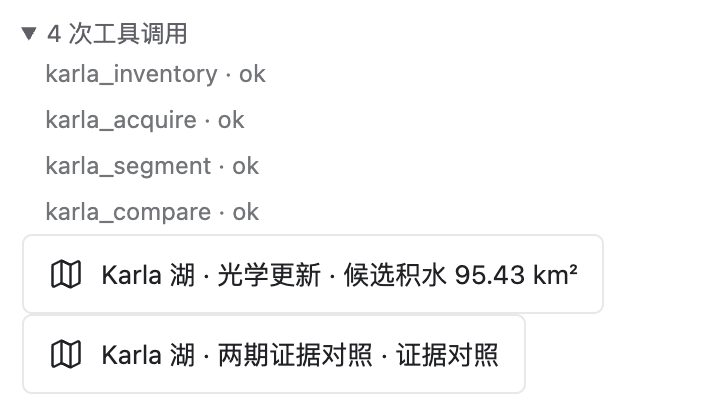
\includegraphics[width=\linewidth]{figures/karla-optical-update.png} &
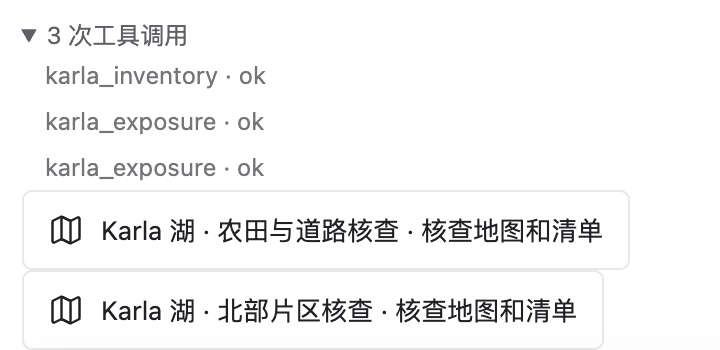
\includegraphics[width=\linewidth]{figures/karla-reuse-exposure.png}
\end{tabular}
\caption{FloodLab 工作台中的真实执行截图，裁切自同一会话的第二、三轮回复，未改动内容。a：下载、分割和对照均有成功记录，下方是光学更新图与两期对照图；b：只有读取已有资料及两次分区核查的记录，各自对应一个成果入口。}
\label{fig:karla-workbench-traces}
\end{figure}


\begin{table}[htbp]
\centering
\caption{三轮工具调用的决策参数与产物。完整记录见成果包。}
\label{tab:karla-turns}
\small
\begin{tabularx}{\linewidth}{@{}>{\raggedright\arraybackslash}p{22mm}>{\raggedright\arraybackslash}p{60mm}>{\raggedright\arraybackslash}X@{}}
\toprule
轮次 & 模型调用的关键参数 & 工具结果\\
\midrule
18 日初报（3 次） & \code{sensor=sar}；\code{algorithm=sar_change}。选法理由附同轨 7 和实际覆盖。 & 在线下载；候选 71.1892 \km，333 个矢量斑块。\\
19 日更新（4 次） & \code{sensor=optical}；\code{algorithm=optical_mndwi}；对照函数收到雷达和光学两个掩膜 ID。 & 在线下载；光学候选 95.4260 \km、126 个斑块；另有一张对照图。\\
分区核查（3 次） & 两次传入同一 \code{comparison_id}，分别设 \code{scope=study}、\code{scope=north}。 & 两套清单，159 和 103 个路段片段；下载、分割调用各为 0。\\
\bottomrule
\end{tabularx}
\end{table}

\begin{figure}[H]
\centering
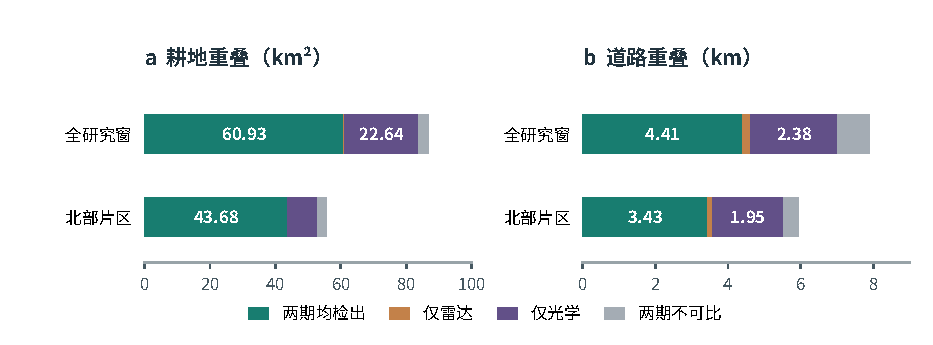
\includegraphics[width=\linewidth]{figures/karla-screening.pdf}
\caption{全研究窗和北部片区的暴露核查。a：耕地重叠面积；b：所选 OSM 道路中心线重叠长度。紫色为单期光学线索，灰色为两期不可比。全窗包含北部片区。}
\label{fig:karla-screening}
\end{figure}

\paragraph{新增观测改变了什么。}
图~\ref{fig:karla-compare} 显示两期均检出 66.9064 \km，仅雷达 1.1196 \km、仅光学 28.5196 \km，另有 23.2508 \km 不可跨期比较。其中 3.1632 \km 在初报中有雷达候选，但缺少可用的光学判读，归入不可比。共同可判读区内，雷达初报涉及 68.0260 \km；光学更新将其中 66.9064 \km 标为两期均检出，并补充只由光学发现的核查线索。与官方同日轮廓的交并比分别为 0.736 和 0.935，反映与基于同批观测制作的参考图之间的空间一致性。

\paragraph{核查名单怎样变化。}
图~\ref{fig:karla-screening} 量化证据更新对清单的影响：全窗仅光学的部分对应额外 22.64 \km 耕地和 2.38 km 道路线索，仍需按单期证据核查。缩小到北部后，约 0.41 km 所选道路处于两期不可比区，应保留为未知。表~\ref{tab:karla-shortlist} 将这种区别落实到路段：两期均检出可优先核对通行记录，单期线索应复判原片，不可比则需补观测。完整清单可通过对应专题图（图~\ref{fig:karla-exposure}）和 CSV 定位；重叠不等于灾时道路封闭。

\begin{table}[H]
\centering
\caption{北部核查清单摘录，按证据类别各取第一条。编号和坐标可在清单及 QGIS 中定位。}
\label{tab:karla-shortlist}
\small
\begin{tabularx}{\linewidth}{@{}p{23mm}p{26mm}r>{\raggedright\arraybackslash}p{36mm}>{\raggedright\arraybackslash}X@{}}
\toprule
证据类别 & OSM way ID & 米 & 中点经纬度（东、北） & 建议核查\\
\midrule
两期均检出 & 538784698 & 865.50 & 22.685619, 39.588435 & 优先核对通行记录\\
仅光学 & 425625350 & 511.06 & 22.720085, 39.555781 & 查影像原片与日期\\
仅雷达 & 538784696 & 24.08 & 22.692878, 39.591697 & 核对该段散射条件\\
两期不可比 & 169155643 & 387.18 & 22.715405, 39.595497 & 补充观测，不作判断\\
\bottomrule
\end{tabularx}
\end{table}

\paragraph{成果验收。}
独立程序核对了像元与矢量面积、证据分类和路段长度，五份 QGIS 工程均通过打开检查。

\clearpage
\begin{landscape}
\thispagestyle{empty}
\noindent\begin{minipage}[c][148mm][c]{\linewidth}
\centering
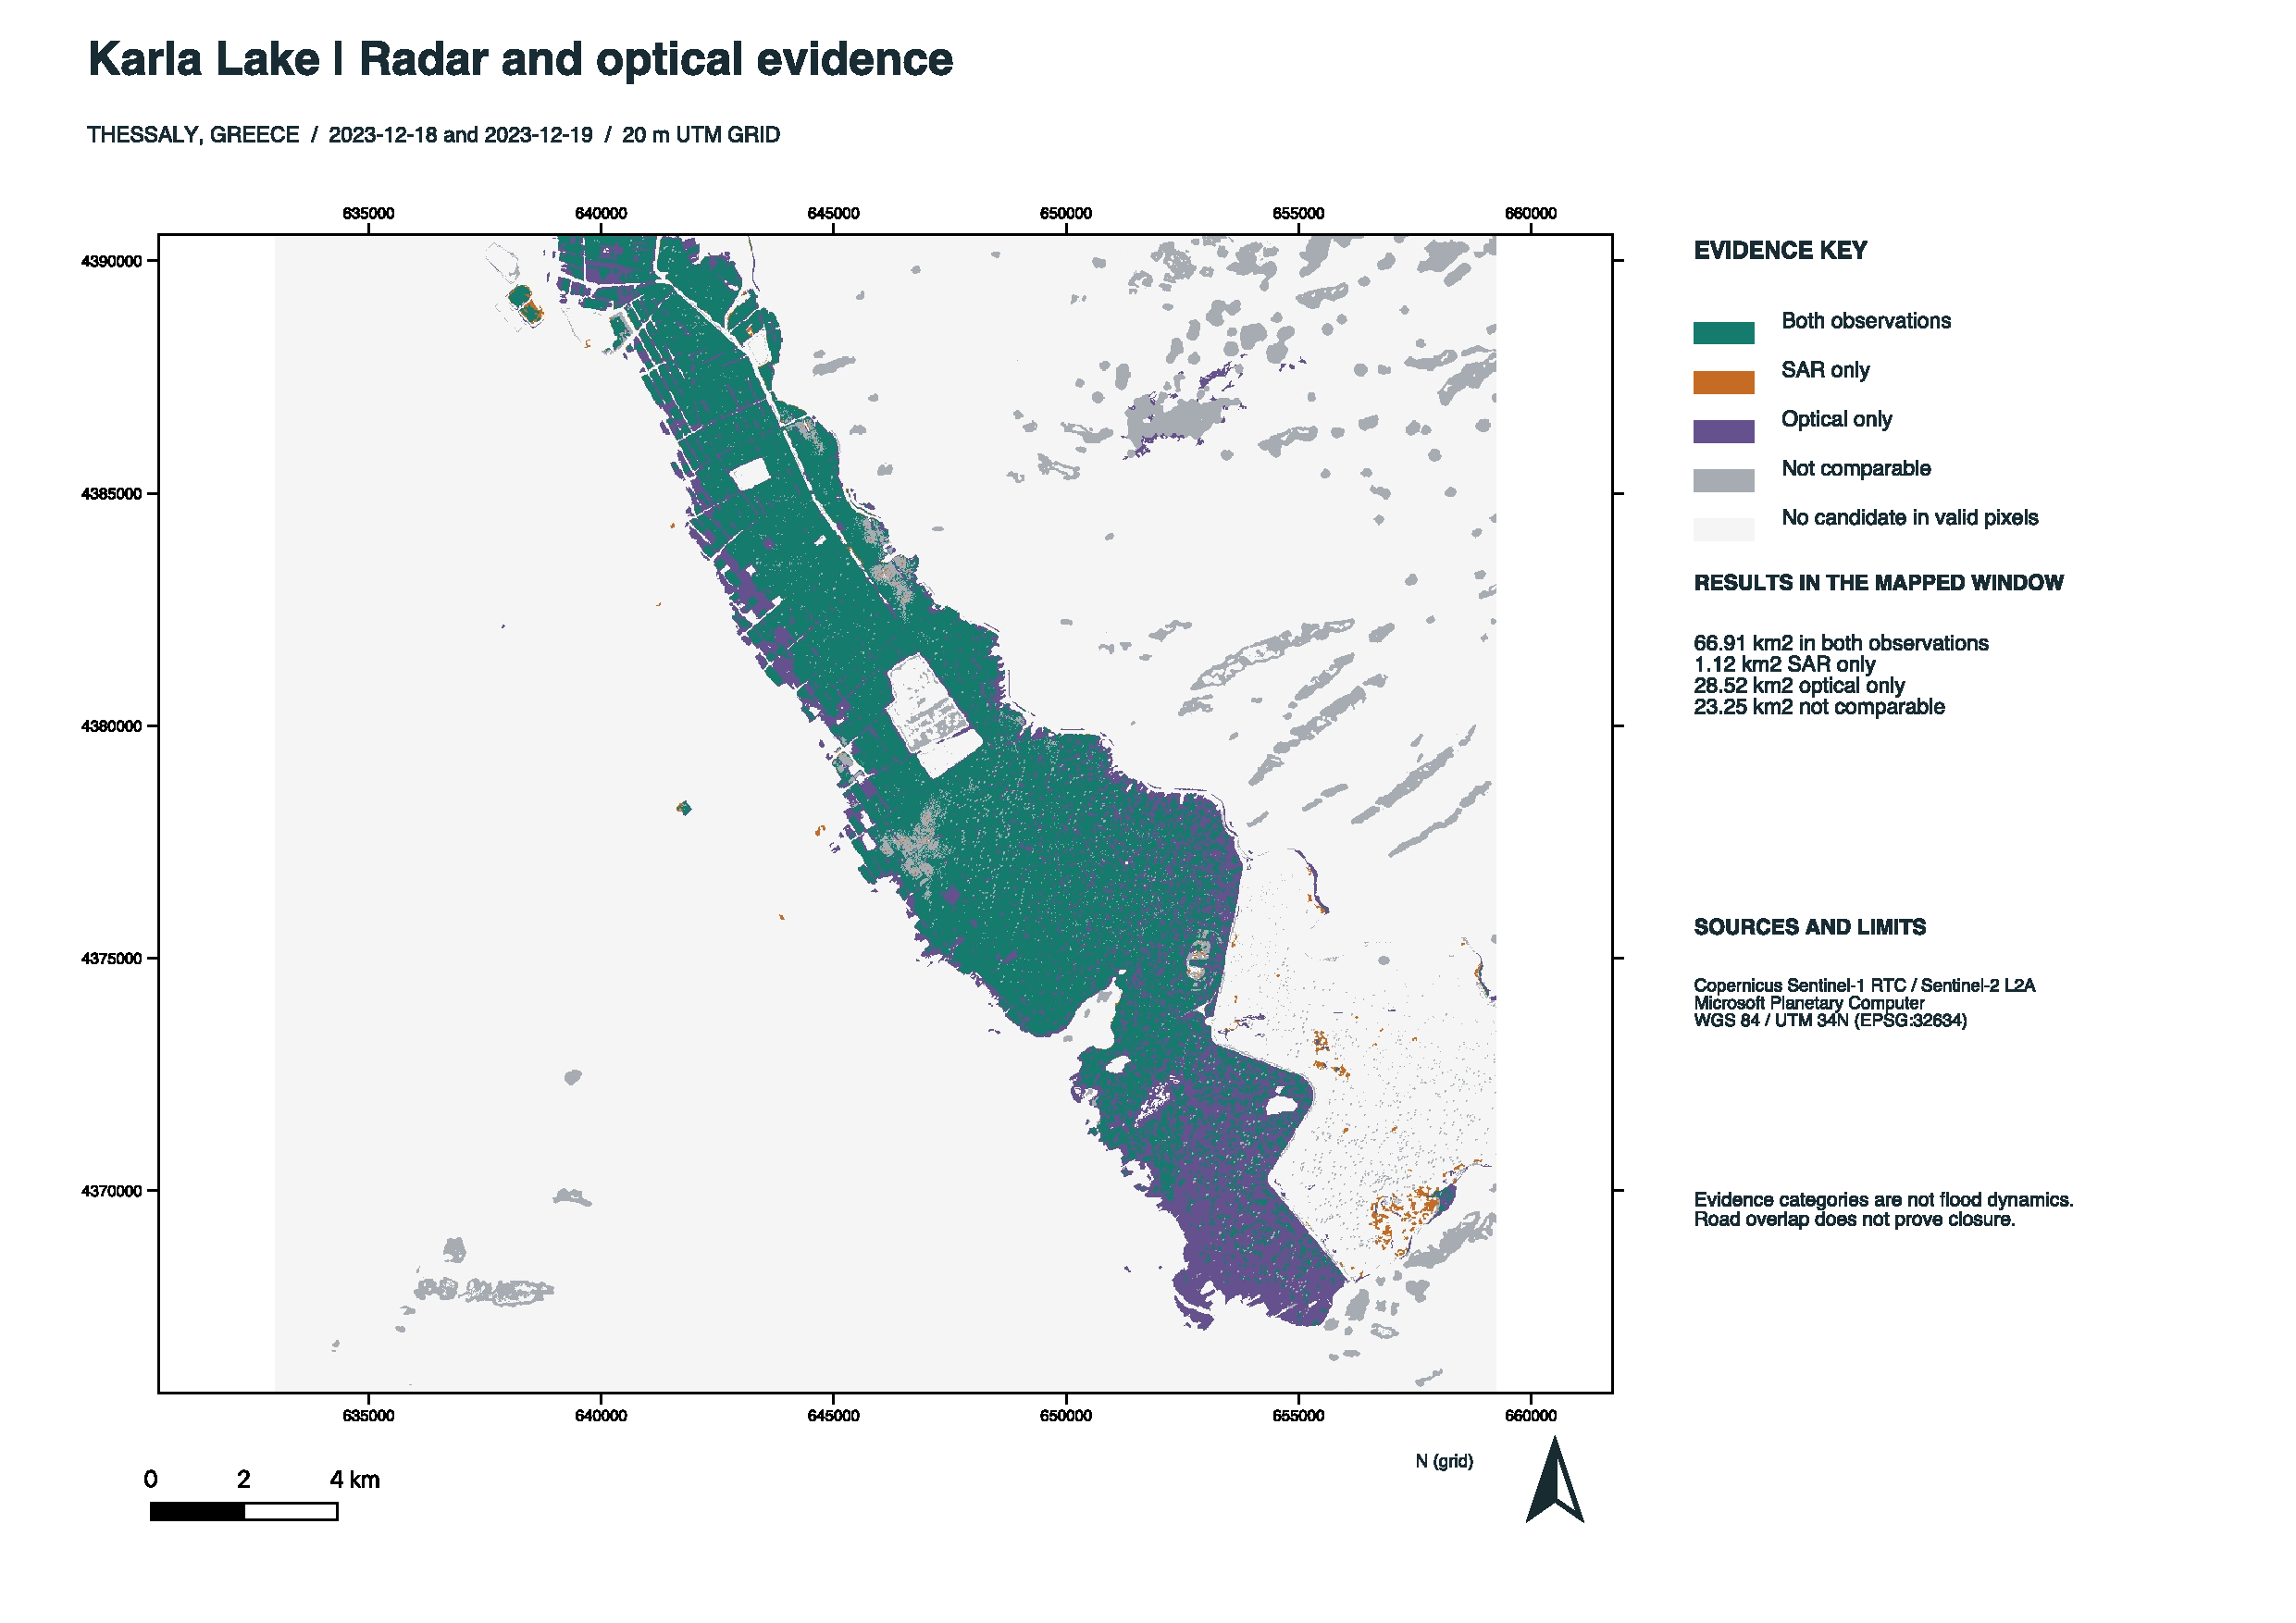
\includegraphics[width=\linewidth,height=136mm,keepaspectratio]{evidence/karla/outputs/comparison-ce8daf32d0/map.pdf}
\captionsetup{hypcap=false}
\captionof{figure}{Karla 湖两期遥感证据对照。灰色表示两期不可比的像元。}
\label{fig:karla-compare}
\end{minipage}\par
\noindent\hfill{\sffamily\small\color{reportmuted}\thepage}\hfill\mbox{}
\end{landscape}

\begin{landscape}
\thispagestyle{empty}
\noindent\begin{minipage}[c][148mm][c]{\linewidth}
\centering
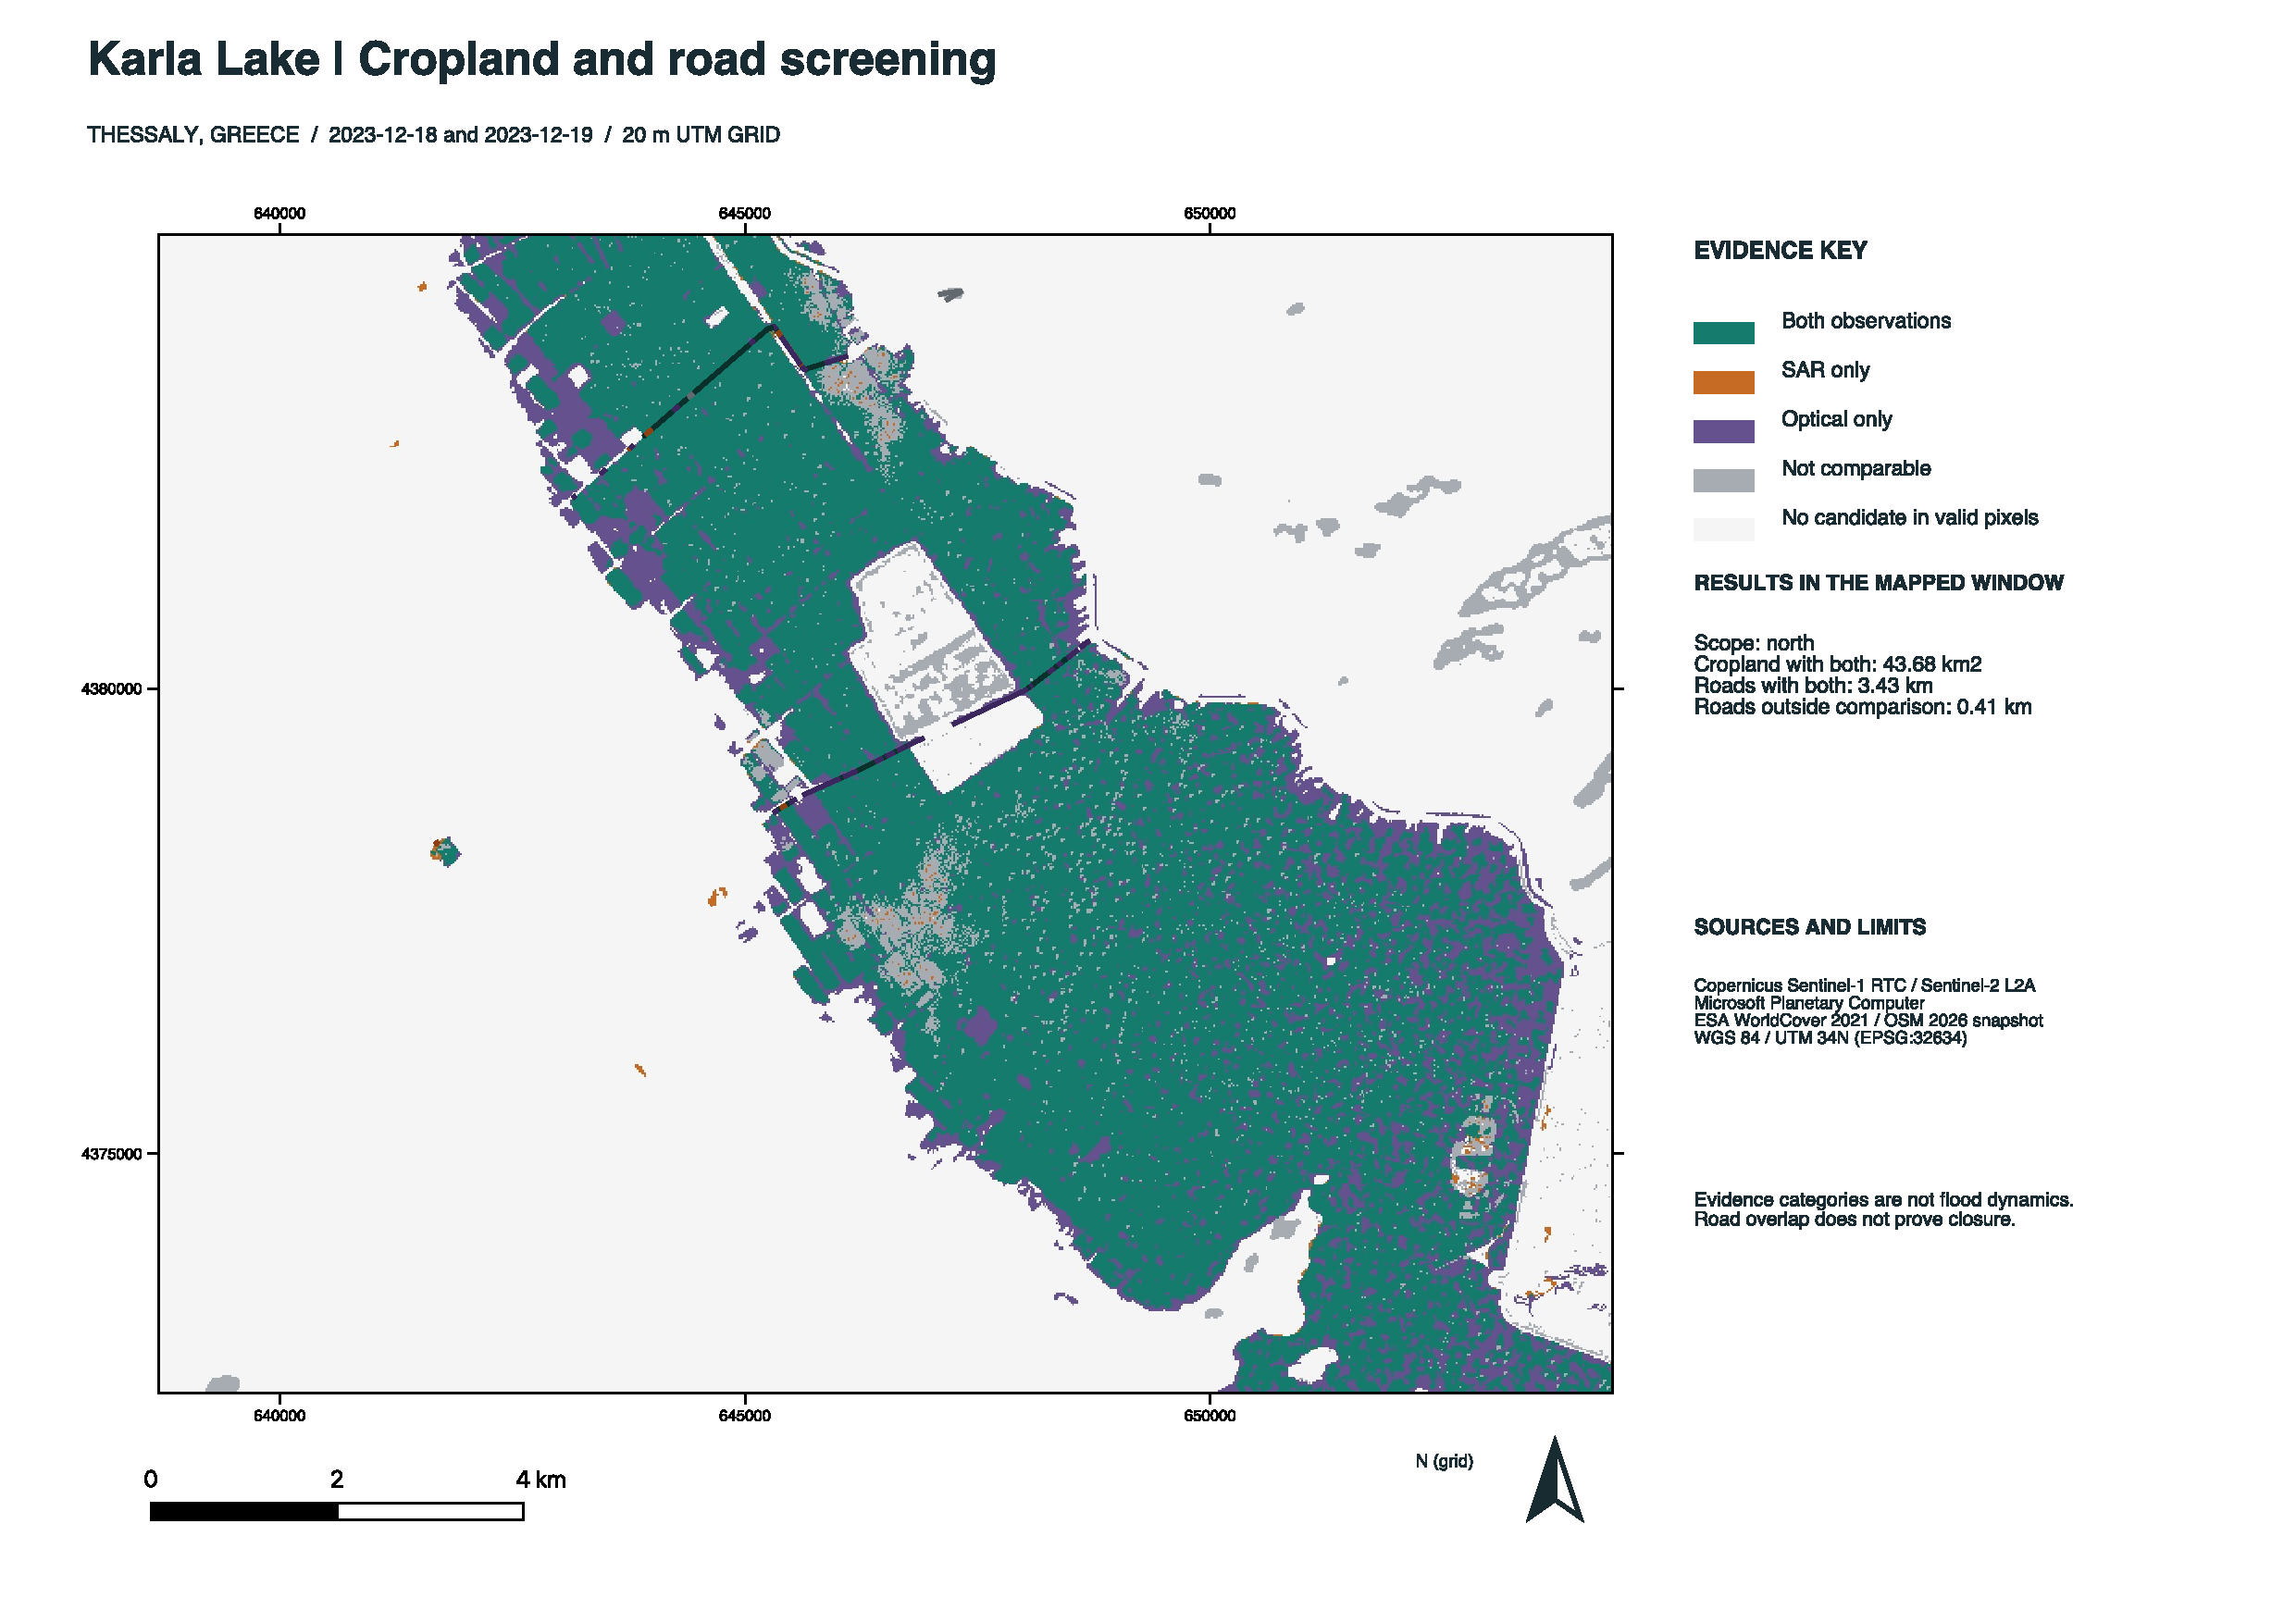
\includegraphics[width=\linewidth,height=136mm,keepaspectratio]{evidence/karla/outputs/exposure-4fa28e86a4/map.pdf}
\captionsetup{hypcap=false}
\captionof{figure}{Karla 湖北部片区核查图。配套清单提供路段中点、重叠长度及证据类别。道路使用 2026 年 OSM 快照。}
\label{fig:karla-exposure}
\end{minipage}\par
\noindent\hfill{\sffamily\small\color{reportmuted}\thepage}\hfill\mbox{}
\end{landscape}

\subsection{扩展案例：三轮洪涝交通核查}
瓦伦西亚案例在同一对话中先筛查区域主干路，再将范围缩小到 Paiporta 和 Benetússer，最后应追问单独核查 Benetússer 的本地道路。每轮由 Pi 传入对应市镇和道路类别，调用空间分析和制图工具。工作台保存各轮地图、路段清单与分析编号。

\begin{table}[H]
\centering
\caption{道路核查三轮的范围、参数和结果。长度为分析支持域内的道路中心线；片段数不是道路条数。}
\label{tab:transport-turns}
\small
\begin{tabularx}{\linewidth}{@{}p{25mm}>{\raggedright\arraybackslash}X r r r@{}}
\toprule
任务 & 实际参数与分析范围 & 片段 & 淹没区（m） & 洪水痕迹（m）\\
\midrule
区域主干路 & 18 个相交候选市镇，17 个有联合资料覆盖；八类干线及连接道 &241&19.67&22\,436.27\\
两市镇主干路 & Paiporta 与 Benetússer；保持来源及类别不变 &23&0.00&2\,002.67\\
本地道路 & 仅 Benetússer；另起本地道路口径 &46&0.00&2\,091.04\\
\bottomrule
\end{tabularx}
\end{table}

\paragraph{第一轮：区域主干路筛查。}
表~\ref{tab:transport-turns} 第一轮纳入 141.66 km 道路中心线。10 个市镇有道路与洪涝证据重叠，累计 241 个片段。淹没区重叠 19.67 m，位于 Picanya 的 CV-36；另有约 22.44 km 与洪水痕迹重叠。约 372 m 带桥隧标记，供后续核对结构高程。空间分布见图~\ref{fig:transport-region}。

例如，Catarroja 的 V-31 有一段约 735.49 m 的洪水痕迹重叠，中心点为西经 $0.389512^\circ$、北纬 $39.396884^\circ$。地图编号对应路段清单中的位置，可据此查阅事件档案。

\paragraph{第二轮：缩小到两个市镇。}
两镇均基本处于联合资料覆盖范围内。Paiporta 所选路网长约 6.33 km，与洪水痕迹重叠约 2.00 km；其中 CV-400 为 1\,235.93 m，CV-407 为 699.50 m，位置见图~\ref{fig:transport-focus}。Benetússer 没有符合当轮筛选条件的历史道路，比例留空。

\paragraph{第三轮：改查 Benetússer 本地道路。}
调整道路类别后，Benetússer 纳入 18.62 km 本地道路，其中约 2.09 km 与洪水痕迹重叠，占 11.23\%，共 46 个片段。按道路名称汇总，Carrer del Moll de l'Estació 重叠 488.90 m；按单个片段排序，Carrer del Mont Alt 最长，为 376.41 m。成果可按道路汇总，也可按片段定位（图~\ref{fig:transport-local}）。

\clearpage
\begin{landscape}
\thispagestyle{empty}
\noindent\begin{minipage}[c][148mm][c]{\linewidth}
\centering
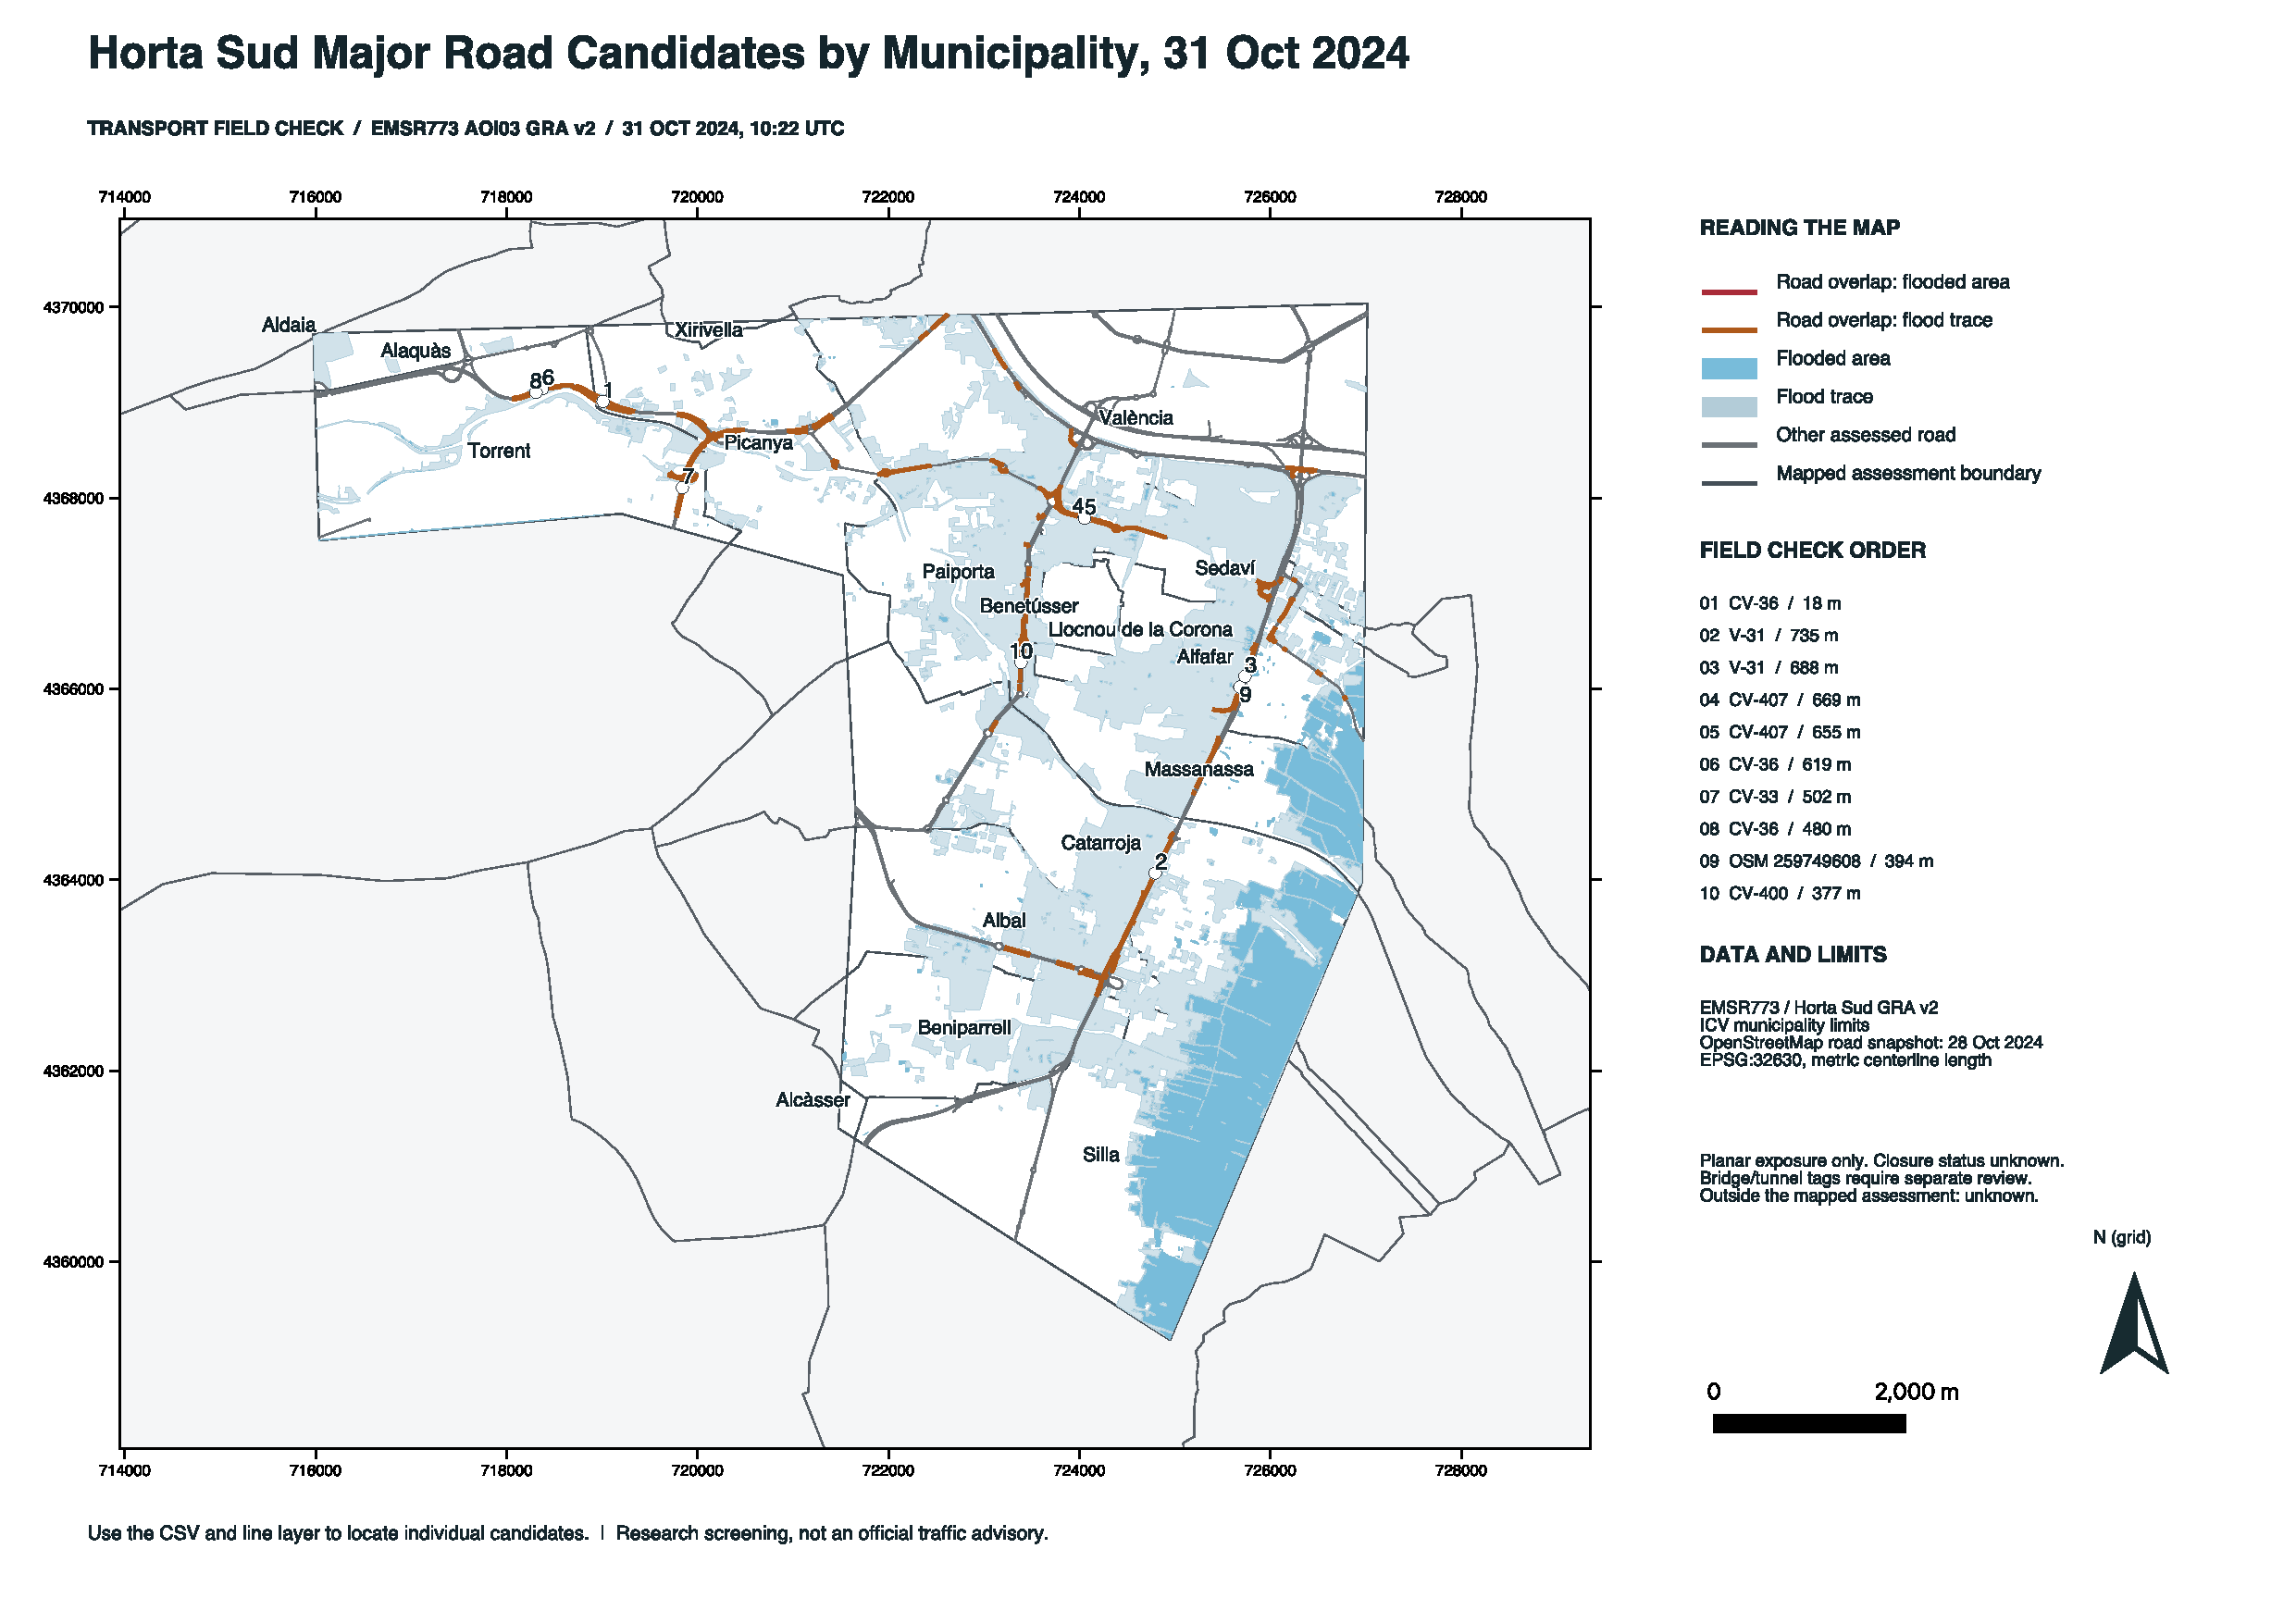
\includegraphics[width=\linewidth,height=136mm,keepaspectratio]{evidence/monitoring/transport/outputs/horta_sud_major_roads_by_town_01/transport.pdf}
\captionsetup{hypcap=false}
\captionof{figure}{Horta Sud 区域主干道路初筛。红色和棕色线段分别表示与观测淹没区和洪水痕迹重叠的道路片段；浅灰标示资料范围外及边界背景。}
\label{fig:transport-region}
\end{minipage}\par
\noindent\hfill{\sffamily\small\color{reportmuted}\thepage}\hfill\mbox{}
\end{landscape}

\begin{landscape}
\thispagestyle{empty}
\noindent\begin{minipage}[c][148mm][c]{\linewidth}
\centering
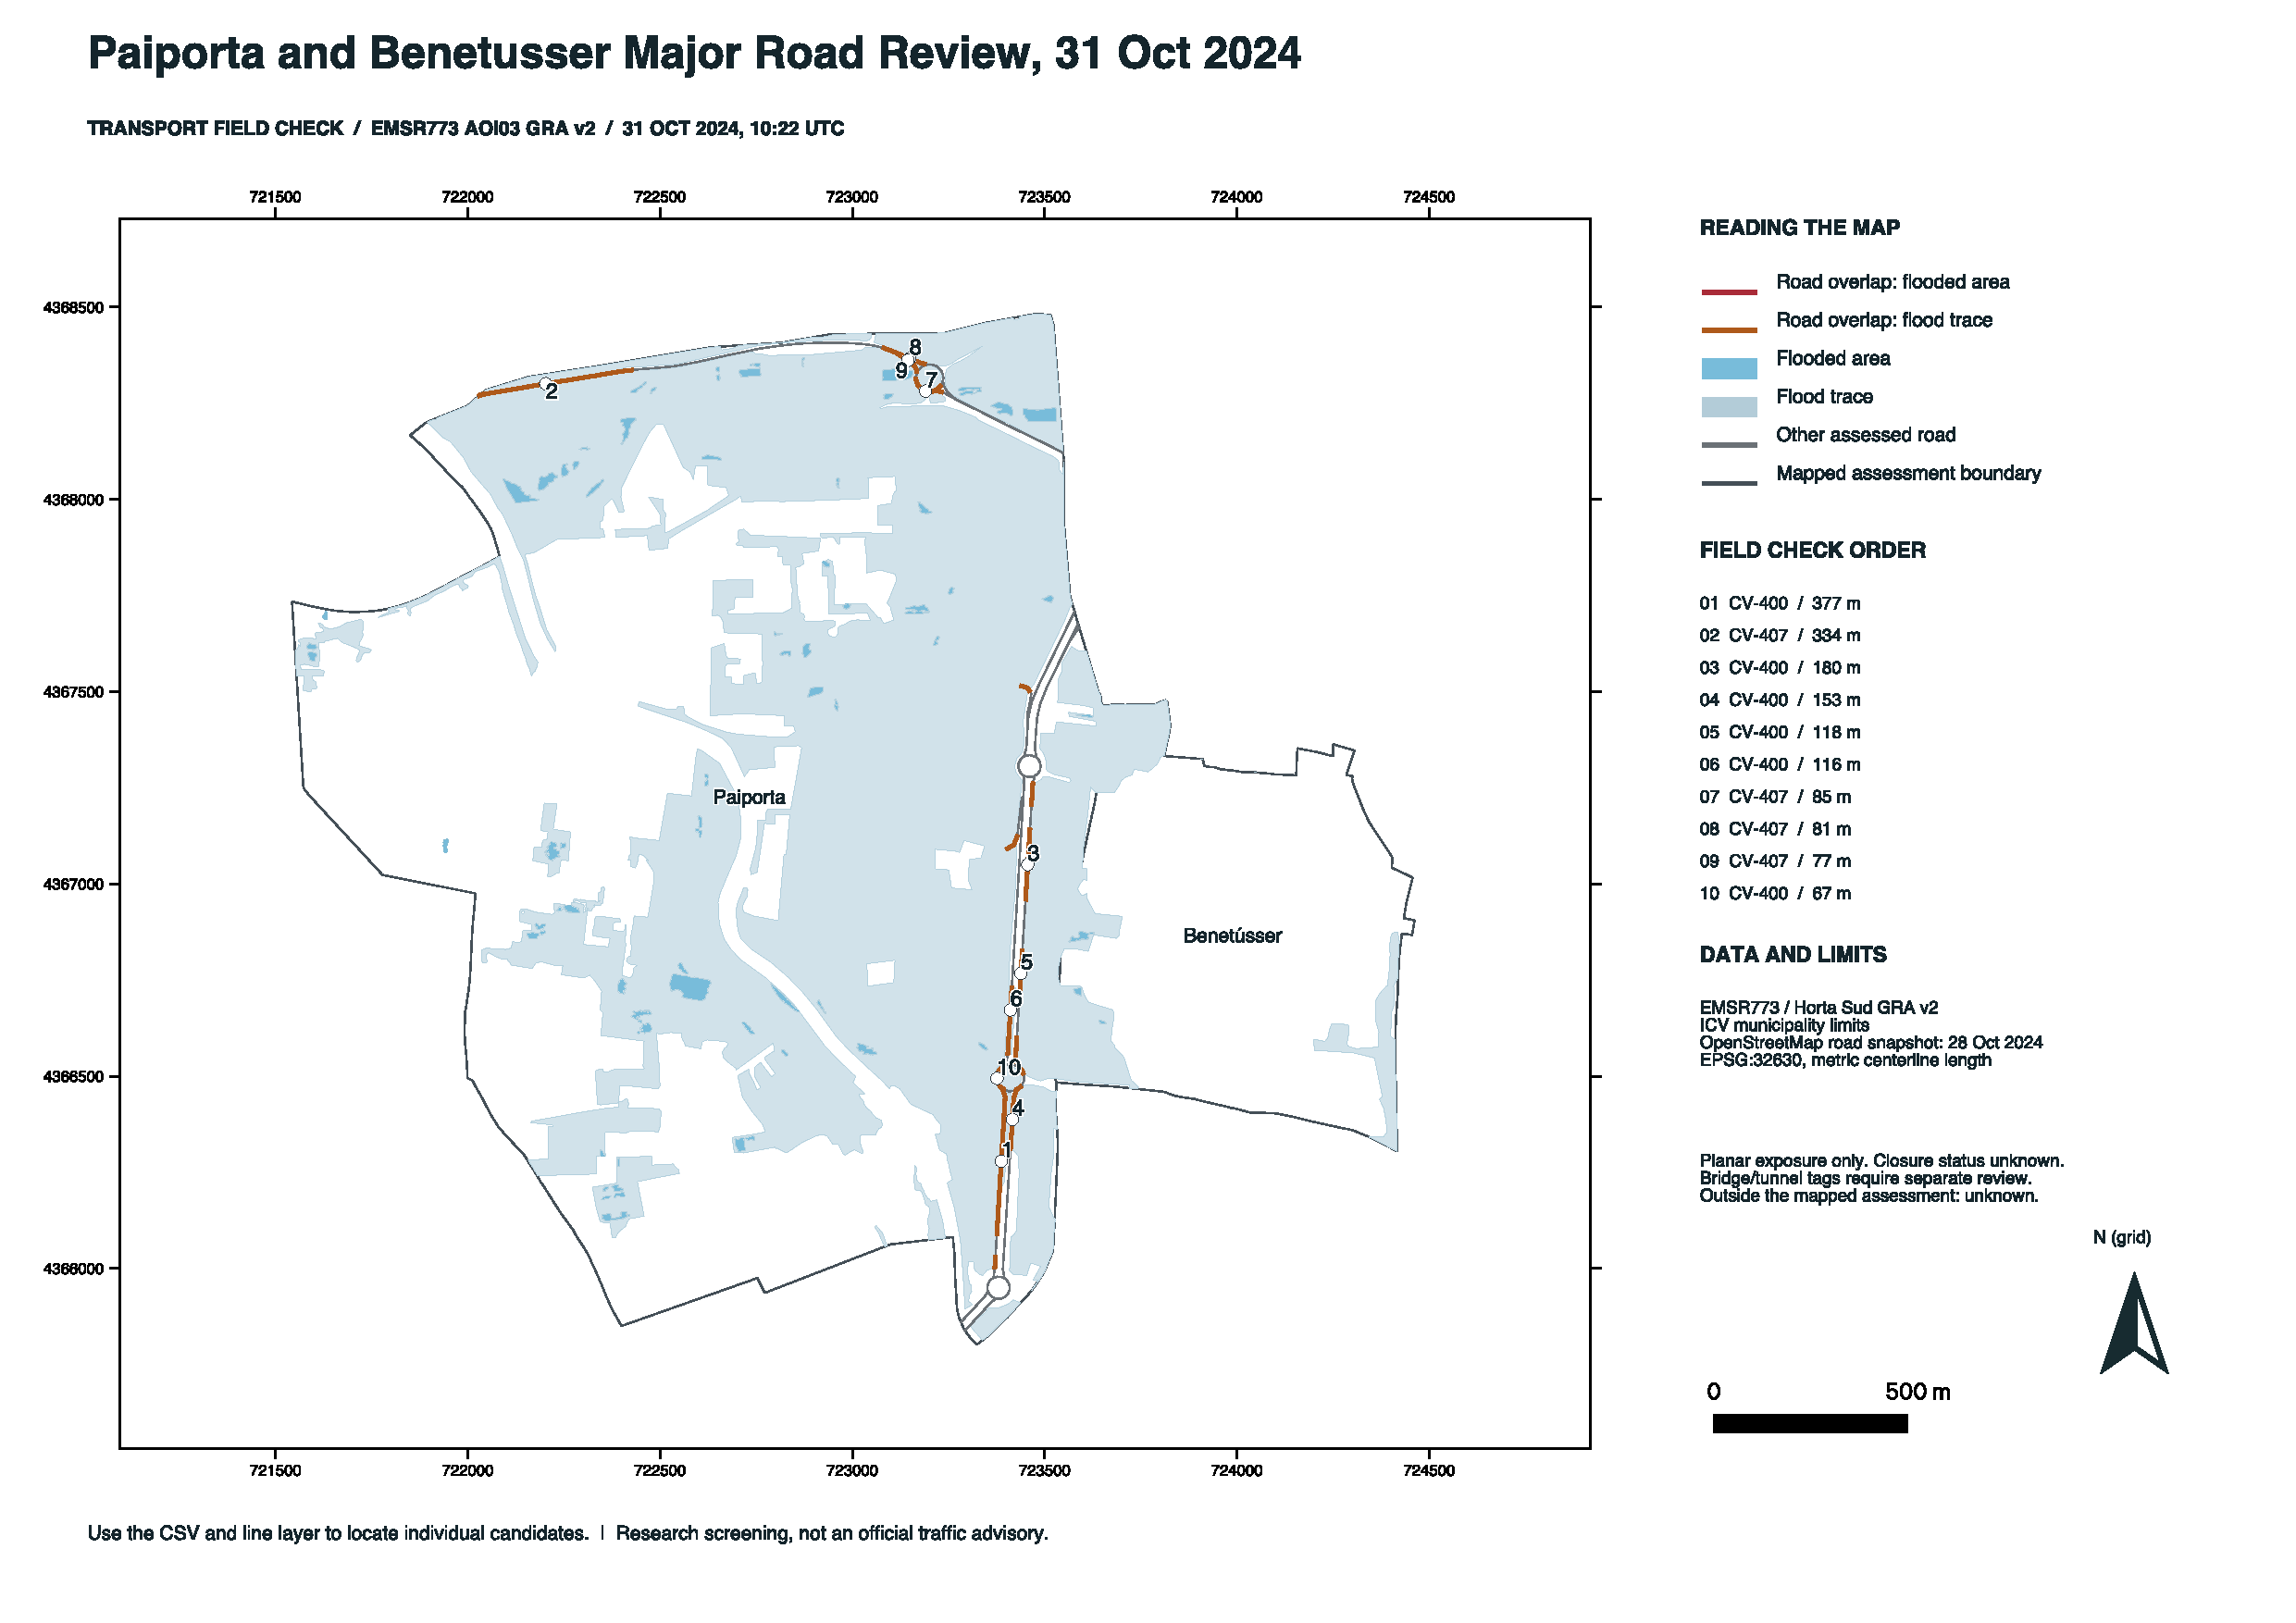
\includegraphics[width=\linewidth,height=136mm,keepaspectratio]{evidence/monitoring/transport/outputs/horta_sud_paiporta_benetusser_major_roads_02/transport.pdf}
\captionsetup{hypcap=false}
\captionof{figure}{Paiporta 与 Benetússer 主干道路核查。沿用区域初筛的资料和道路类别，编号为本轮候选片段的核查次序。}
\label{fig:transport-focus}
\end{minipage}\par
\noindent\hfill{\sffamily\small\color{reportmuted}\thepage}\hfill\mbox{}
\end{landscape}

\begin{landscape}
\thispagestyle{empty}
\noindent\begin{minipage}[c][148mm][c]{\linewidth}
\centering
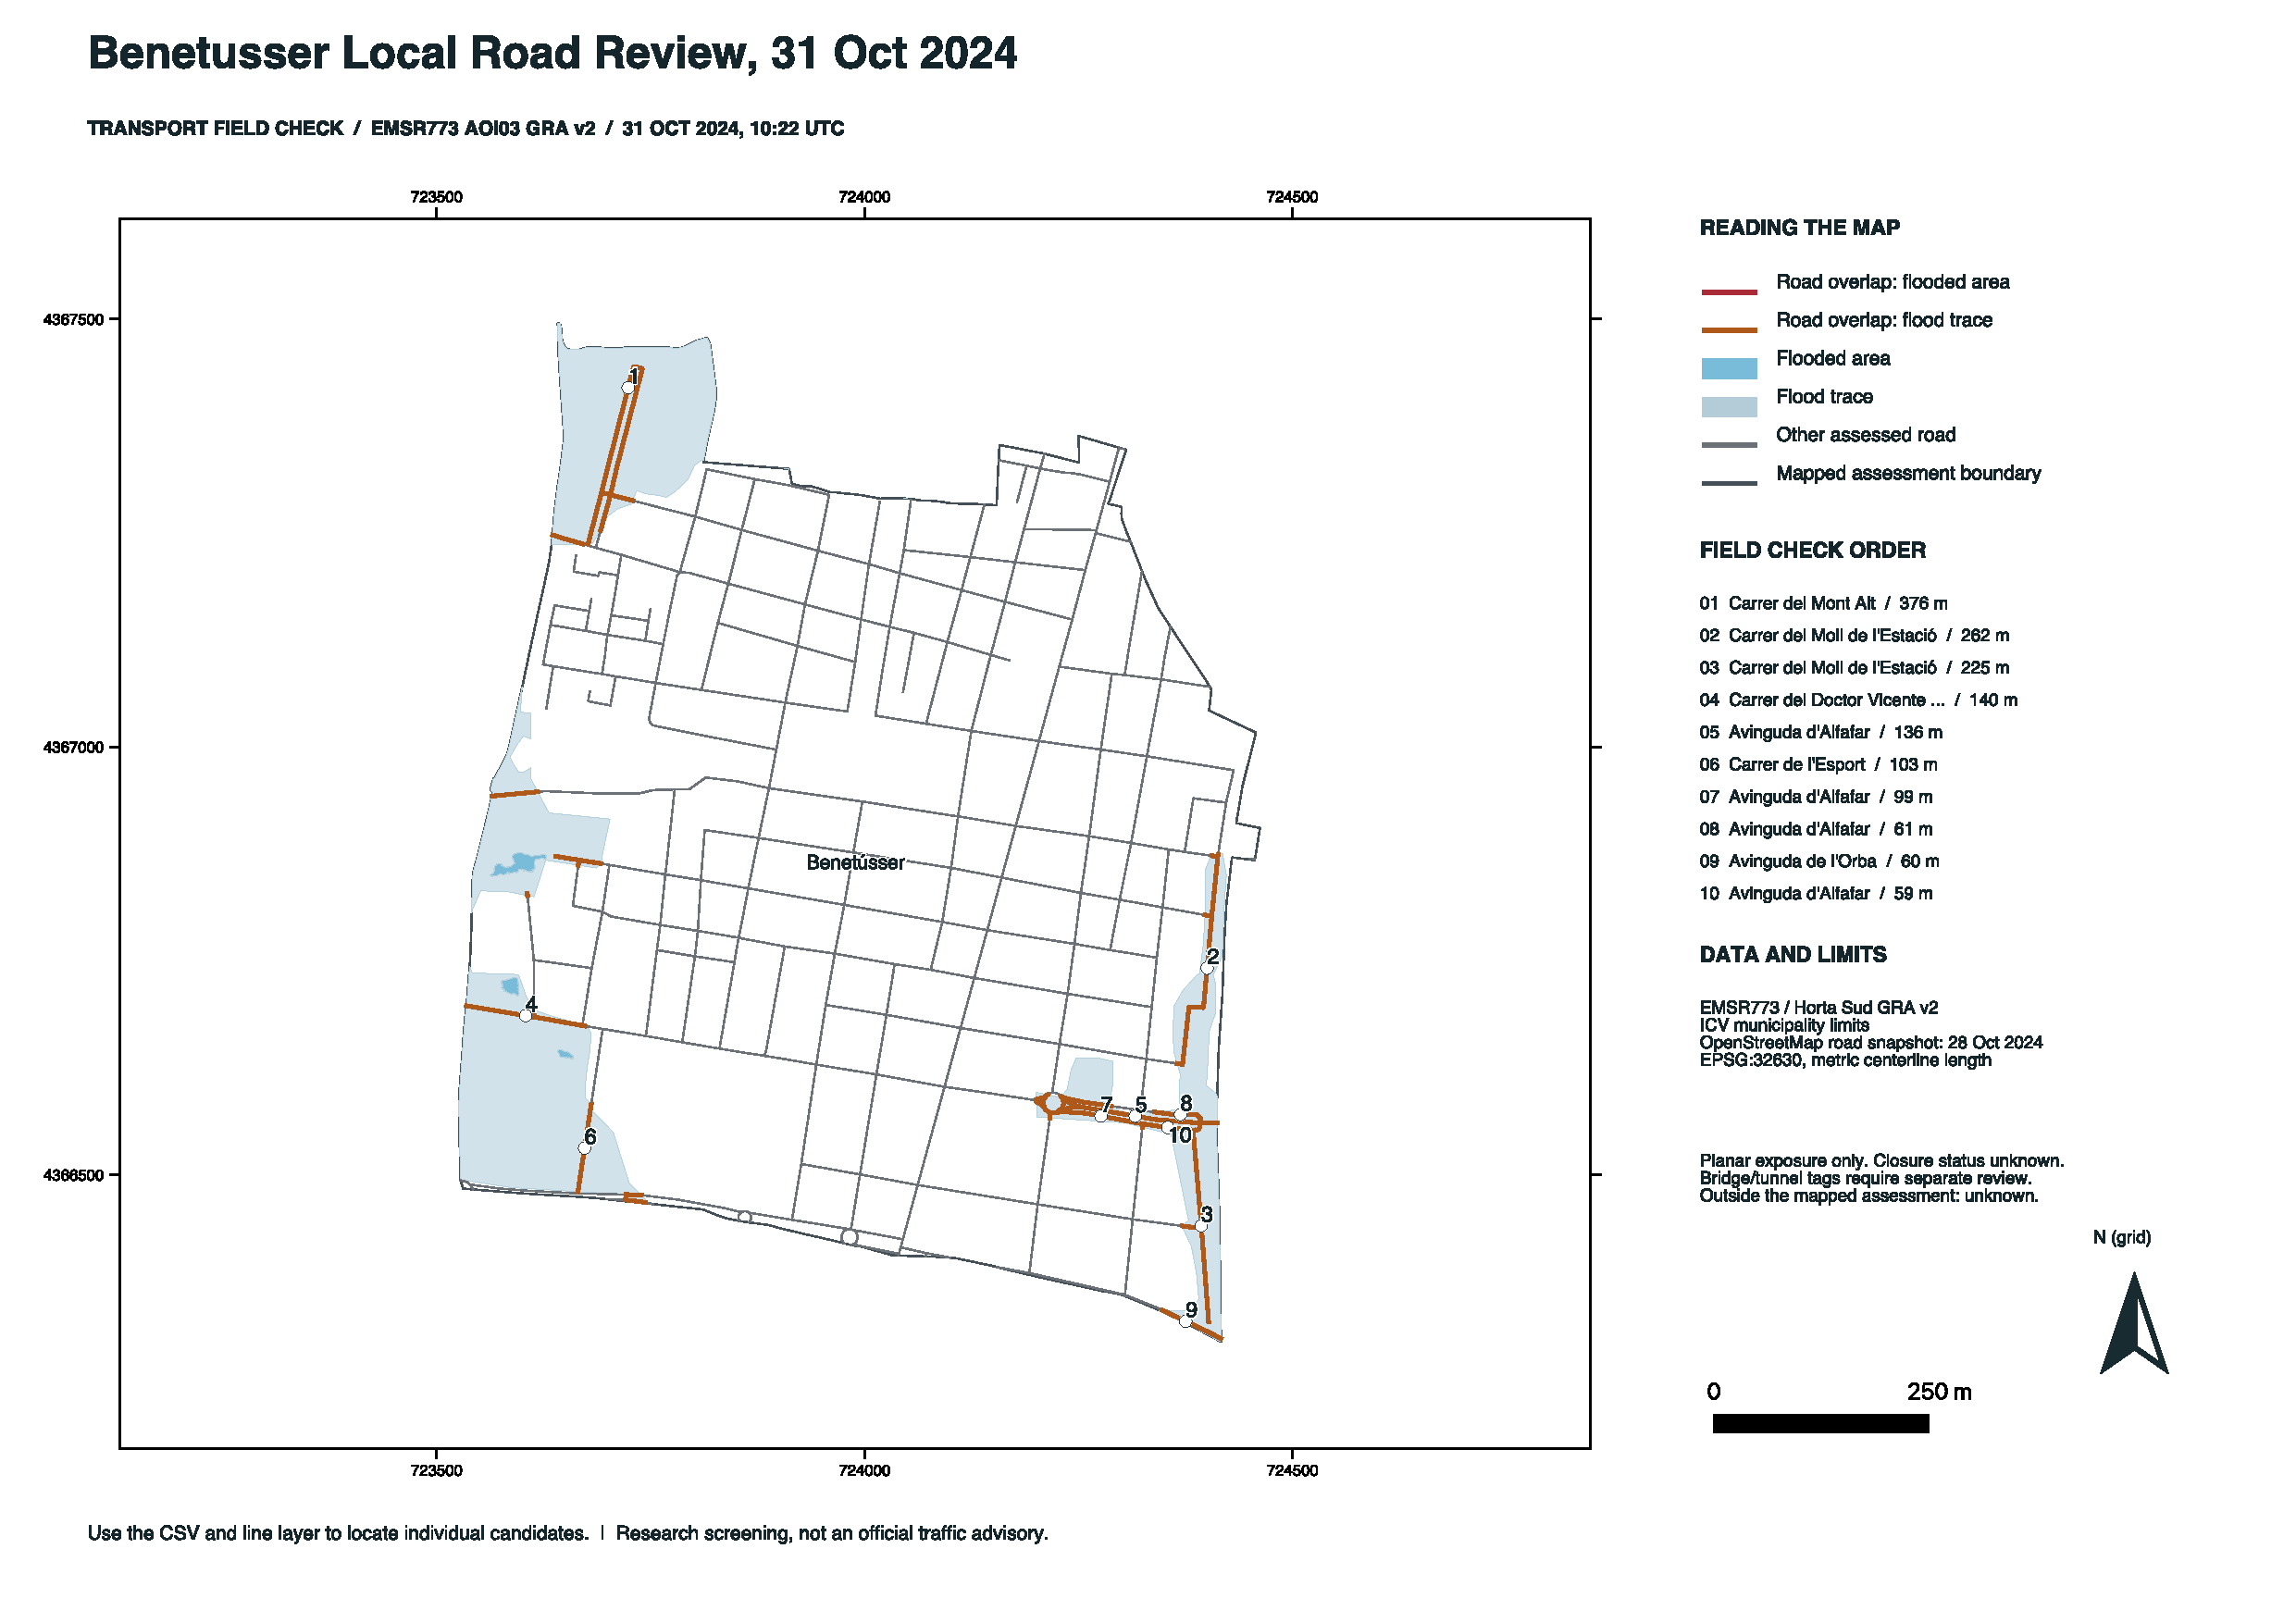
\includegraphics[width=\linewidth,height=136mm,keepaspectratio]{evidence/monitoring/transport/outputs/horta_sud_benetusser_local_roads_03/transport.pdf}
\captionsetup{hypcap=false}
\captionof{figure}{Benetússer 本地道路复核图。与前图相比，研究问题改为四类本地道路；棕色路段只表示与洪水痕迹重叠。}
\label{fig:transport-local}
\end{minipage}\par
\noindent\hfill{\sffamily\small\color{reportmuted}\thepage}\hfill\mbox{}
\end{landscape}


\subsection{工程回归：道路类别与网格尺寸变更}
在市镇核查之外，另用全道路 1 km、四类主干道路 2 km 和住宅道路 500 m 三种设置检查通用工具。表~\ref{tab:product-runs} 中 822 格均通过逐格复算。道路类别和分辨率改变后，系统重新筛选道路、生成网格并导出成果。

\begin{table}[htbp]
\centering
\caption{三种道路类别与网格尺度下的统计与复算结果。}
\label{tab:product-runs}
\small
\begin{tabular*}{\linewidth}{@{\extracolsep{\fill}}lrrrr@{}}
\toprule
道路条件与网格 & 格数 & 总长（m） & 暴露长（m） & 逐格复算\\
\midrule
全部道路 / 1 km &156&1\,298\,372.08&8\,027.37&通过\\
四类主干道路 / 2 km &42&56\,848.18&443.52&通过\\
住宅道路 / 500 m &624&627\,080.26&277.59&通过\\
\bottomrule
\end{tabular*}
\end{table}


\subsection{扩展案例：从非预装观测产品到专题图}
克里特岛 Kastelli 案例检验新地点的数据获取。第一轮要求列出 EMSR933 的可用观测日期，Pi 按请求查询目录；第二轮根据追问下载编号 2962、观测时间为 2026 年 10 月 6 日 10:47 的产品并量算。

QGIS 在等积投影 EPSG:6933 中合并 88 个多边形，得到 0.241266 \km 的积水及洪水痕迹并集。1 km 网格中有 20 格与之相交；相交最多的 8-11 格为 0.071973 \km，占完整网格的 7.20\%。网格合计与并集面积已核对，分布见图~\ref{fig:kastelli}。

\begin{figure}[htbp]
\centering
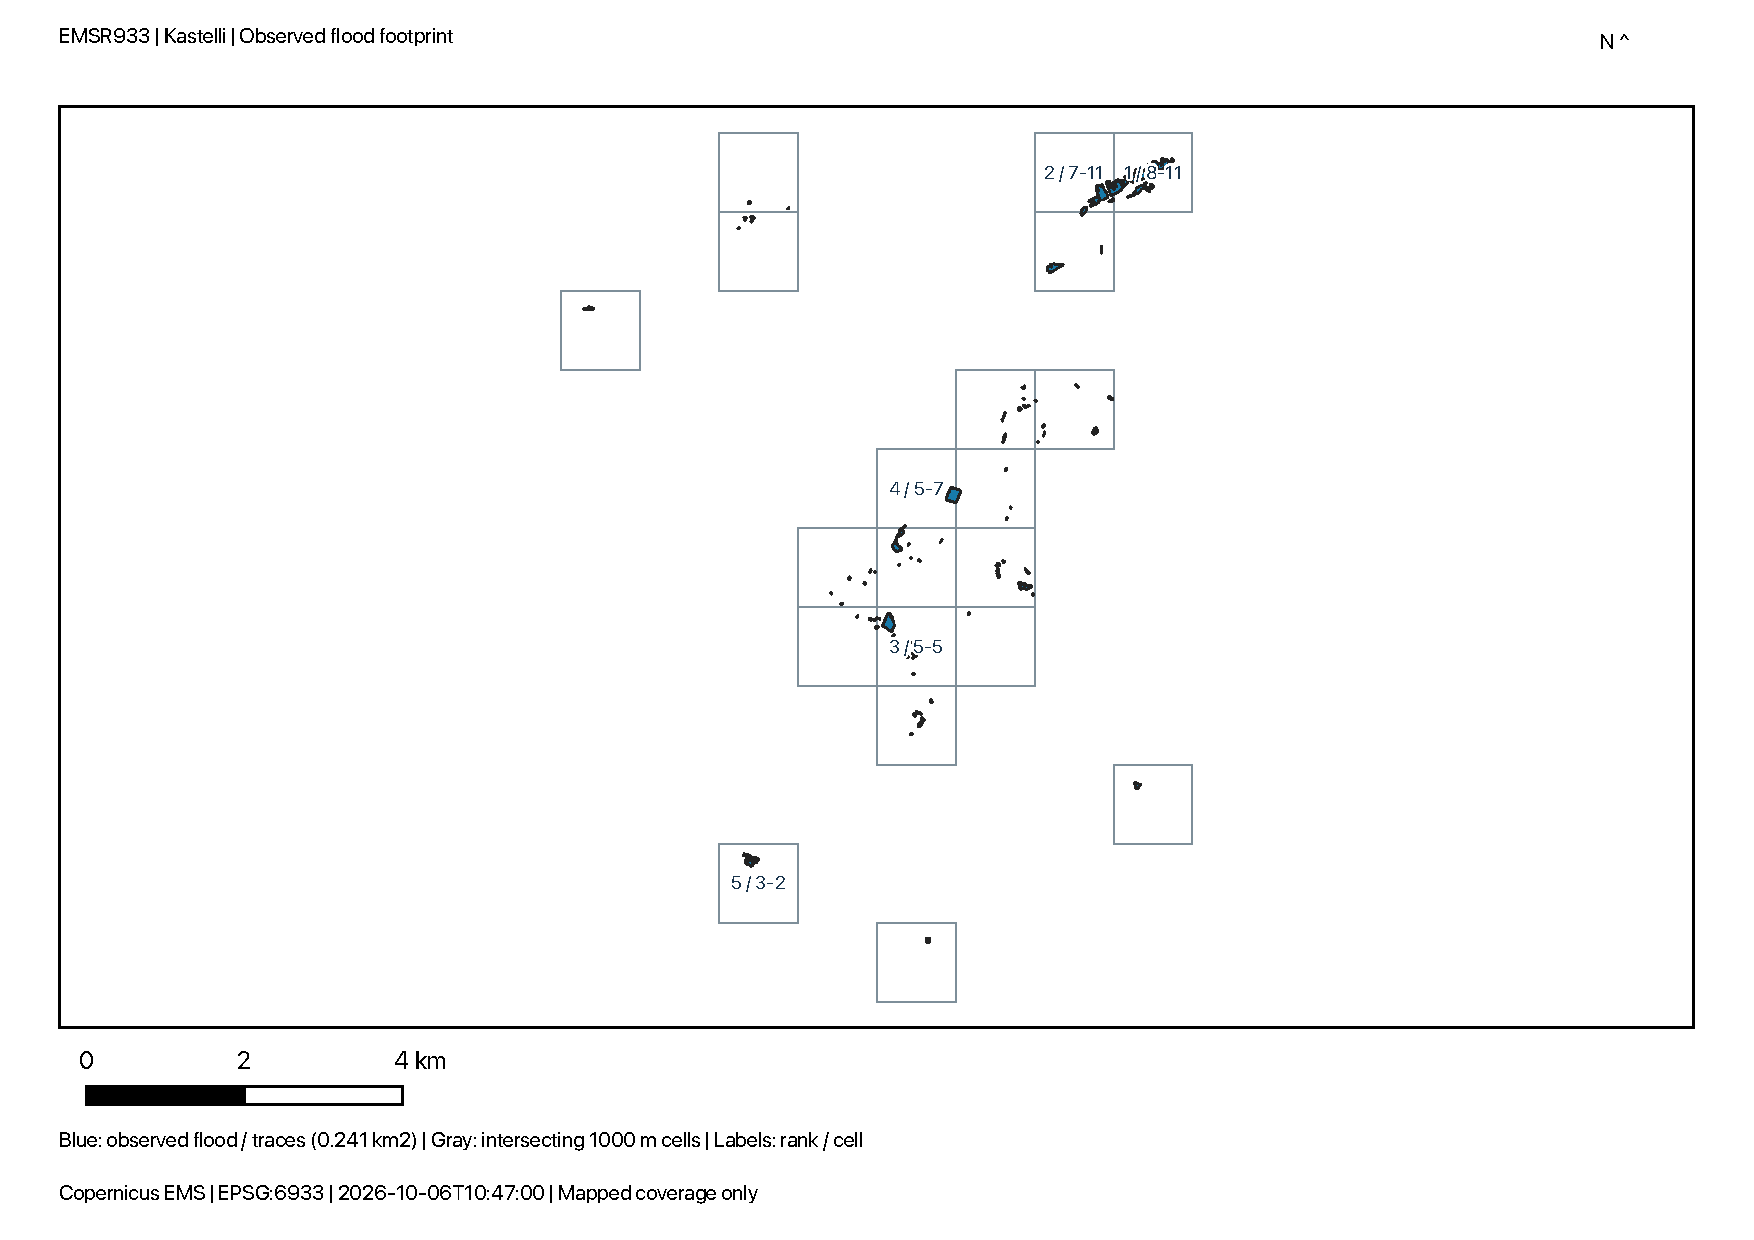
\includegraphics[width=.98\linewidth]{evidence/monitoring/crete/outputs/EMSR933-2962-07ce5273/map.pdf}
\caption{Kastelli 官方观测轮廓及 1 km 统计网格。深色轮廓表示观测产品中的积水及洪水痕迹；标注为排名和格号。完整图及可编辑工程随成果归档。}
\label{fig:kastelli}
\end{figure}

\subsection{补充能力：模糊提问与观测目录}
遇到“最近国内哪儿发生洪涝”一类请求，Pi 先按时间窗和地点查询新闻或事件目录，列出带来源的候选，再协助用户选择查看资料、量算面积或分析道路。

莆田--仙游案例查询了 2026 年 9 月 3 至 6 日（当地时间）的指定检索框：目录未返回匹配的 Sentinel-1 条目，返回同一次过境的 4 个 Sentinel-2 瓦片，整景云量字段均为 100\%。系统保存查询元数据和足迹，并生成影像覆盖图（图~\ref{fig:coverage}），供进一步判断是否值得下载像元。

\begin{figure}[htbp]
\centering
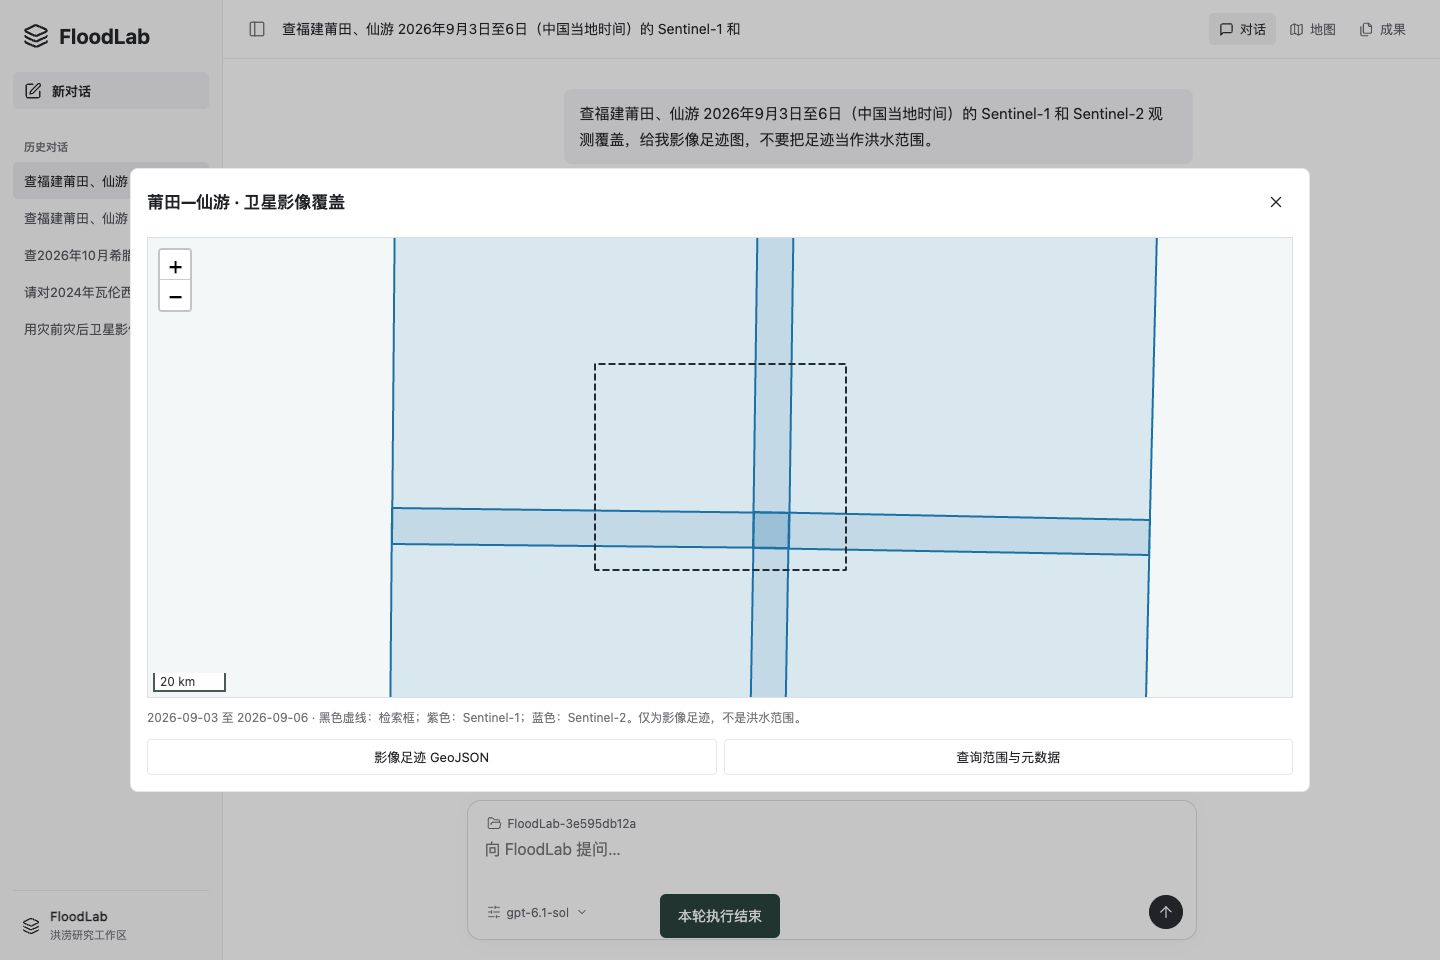
\includegraphics[width=.91\linewidth,trim=125 35 125 35,clip]{evidence/monitoring/runs/putian-1-map.png}
\caption{莆田--仙游影像目录覆盖。黑色虚线是检索框，蓝色是 Sentinel-2 影像足迹。}
\label{fig:coverage}
\end{figure}

\subsection{结果分析与核验}
Karla 的核验按三轮交付展开：前两轮分别复核雷达和光学候选的栅格、矢量面积；更新版核对两期证据分类；最后从核查图层重新统计耕地面积和路段长度。五份 QGIS 工程均可重新打开。图~\ref{fig:karla-workbench-traces} 将核验结果落到用户看得见的成果入口。

瓦伦西亚的三轮分析以独立几何程序复算市镇覆盖、道路总长和两类交叠长度。市镇级重叠长度与原结果的最大绝对差小于 $10^{-7}$ m，低于 0.05 m 容差；各轮地图、路段清单和复算记录随成果归档。通用道路实验另核对了三种网格和道路类别。小规模对照中，使用通用工具的流程也能完成指定任务。本实践体现的价值是把资料检查、选法和追问中的成果复用安排在同一工作区，使各轮结果能被检查和继续使用。

\section{总结与反思}
\subsection{实践总结}
本次实践从两类卫星的像元生成独立证据，把观测更新落实成可对照的候选图和核查清单。智能体的作用体现在实际调用：先用雷达完成截止日初报，新影像到达后根据光学覆盖改变方法，最后缩小核查范围并复用已有证据。不同证据不混写成真值，人工可以定位哪一类结论需要补现场记录。瓦伦西亚补充了基于官方现成轮廓的城市交通核查，两套路线的数据、空间支持域和结论边界分别记录。

人工工作贯穿选题、流程设计和复核。讨论中将主案例从单次分割调整为三轮恢复监测，并将道路暴露定义为线与证据范围的平面重叠。成果审阅重点核对观测日期、统计分母、地图图例及路段坐标。项目以 Pi 和 QGIS 执行任务，使用 Codex 辅助开发、测试和报告整理。

\subsection{局限与改进方向}
Karla 两期观测相隔约 29 小时，且使用不同传感器；差异图适合组织核查线索，判断实际洪水扩张或退水还需更密集的同类观测。耕地分类和道路快照来自不同年份，空间重叠用于筛查，评估灾损或封路需补充同期地面资料和通行记录。

后续可在其他事件中用独立标注检验选法与工具链。
